% Submission for the International Journal of Forecasting
% Open-Source Forecasting Special Section
% Template: elsarticle with the IJF model5-names bibliography style.

\documentclass[11pt,3p,review,authoryear]{elsarticle}

\journal{International Journal of Forecasting}
\bibliographystyle{model5-names}
\biboptions{longnamesfirst}

\usepackage{graphicx}
\usepackage{hyperref}
\usepackage{url}
\usepackage{booktabs}
\usepackage{listings}
\usepackage{xcolor}

\definecolor{codegray}{rgb}{0.5,0.5,0.5}
\definecolor{codegreen}{rgb}{0,0.5,0}
\definecolor{codepurple}{rgb}{0.58,0,0.82}

\lstdefinestyle{pystyle}{
    basicstyle=\ttfamily\small,
    commentstyle=\color{codegreen},
    keywordstyle=\color{blue},
    stringstyle=\color{codepurple},
    numberstyle=\tiny\color{codegray},
    showstringspaces=false,
    breaklines=true,
    frame=single,
    language=Python,
    captionpos=b
}
\lstset{style=pystyle}

\graphicspath{{images/}}

\begin{document}

\begin{frontmatter}

\title{Probabilistic Forecasting in the JAX Ecosystem:
NumPyro, Composability, and Community}

%% AUTHORS %%%%%%%%%%%%%%%%%%%%%%%%%%%%%%%%%%%%%%%%%%%%%%%%%%%%%%%%%%%%%%%%%%%%
\author[jo]{Juan Orduz\corref{cor}}
\ead{juan.orduz@pymc-labs.com}
\author[goog]{Du Phan}
% \ead{} % TODO: confirm coauthor email
\author[amzn]{Theo Rashid}
% \ead{} % TODO: confirm coauthor email
\address[jo]{PyMC-Labs}
\address[goog]{Google}
\address[amzn]{Amazon}
\cortext[cor]{Corresponding author.}
%%%%%%%%%%%%%%%%%%%%%%%%%%%%%%%%%%%%%%%%%%%%%%%%%%%%%%%%%%%%%%%%%%%%%%%%%%%%%%%%

\begin{abstract}
Open-source forecasting is often framed as a competition between turn-key libraries that wrap canonical models behind friendly APIs. This paper argues that a second, complementary mode of open-source forecasting deserves attention: composable probabilistic substrates such as NumPyro, layered on top of the JAX ecosystem, where practitioners assemble bespoke models from a small set of primitives. The story is not only about a framework. It is also about the community layer of tutorials, blog posts, and worked examples that bridges the gap between substrate flexibility and practical use. We trace the Pyro lineage that NumPyro inherits, isolate the two primitives that matter most for time series, namely \texttt{scan} for recursive state updates and \texttt{plate} for vectorization across groups, and review the inference toolkit that ties everything together: NUTS for full Bayesian posteriors, stochastic variational inference for scale, and the seamless composition with Optax optimizers. We then survey six case studies that exercise the resulting flexibility: hierarchical pooling for sparse panels, intermittent demand with availability constraints, censored demand under stockouts, Bayesian vector autoregression, Gaussian processes via Hilbert space approximation, and prior calibration through additional likelihoods. We discuss the steep learning curve that comes with this expressive power, the active community effort to lower it through accessible material, and the broader open-source forecasting landscape that the substrate complements rather than replaces.
\end{abstract}

\begin{keyword}
Probabilistic forecasting \sep Bayesian methods \sep Open-source software \sep Hierarchical models \sep Intermittent demand \sep Gaussian processes
\end{keyword}

\end{frontmatter}


% =============================================================================
\section{Introduction}
% =============================================================================

Forecasting drives consequential decisions across retail, energy, finance, public health, and operations research. The decisions that follow a forecast are rarely symmetric in their costs: a stockout differs from overstock, an under-provisioned grid differs from an over-provisioned one, and a missed marketing window differs from an inefficient one. Point forecasts collapse this asymmetry into a single number and force the consumer of the forecast to invent uncertainty after the fact. Probabilistic forecasts, by contrast, carry the uncertainty alongside the prediction and let downstream decision makers reason about quantiles, tails, and joint events in a principled way. A further distinction matters here. A structural Bayesian model yields coherent joint draws from the data-generating process, not merely a collection of marginal quantiles. Sampling whole trajectories exposes scenarios and correlated tail events that median-centered intervals hide, in the same way that the joint scenario draws of a Bayesian election model convey outcomes that marginal summaries obscure \citep{heidemanns2020updated}.

The open-source community has responded to this need with an impressive landscape of forecasting tools. Pre-packaged libraries such as the Nixtla ecosystem and sktime expose canonical statistical and machine-learning methods through friendly user-facing APIs \citep{nixtla2024, loning2019sktime}. GluonTS bundles deep probabilistic forecasters with a consistent training and evaluation harness \citep{alexandrov2020gluonts}. More recently, large pre-trained time-series foundation models such as Chronos and TimesFM offer zero-shot forecasts behind comparably simple interfaces \citep{ansari2024chronos, timesfm_jax}. The classical statistical modeling tradition is well served by statsmodels \citep{statsmodels} and by R libraries that have shaped a generation of forecasting practice \citep{hyndman2021forecasting}. These libraries succeed precisely because they hide model implementation behind a uniform interface and let practitioners focus on data, validation, and deployment.

This paper is concerned with a different layer of the open-source forecasting stack. There is a recurring class of forecasting problems where the canonical model menu is the wrong starting point. Demand series may contain zeros that mix true zero demand with stockout-censored observations. A retailer may want to share information across thousands of related series in ways that respect both group-level and unit-level idiosyncrasies. A practitioner may need full control over how covariates enter the model, encoding holiday and event effects with bespoke shapes, including before-and-after windows, Fourier terms, or bump functions, rather than a single indicator column, while a standard time series component handles the business-as-usual dynamics. An analyst may want to combine a long historical time series with a small number of expert-elicited prior anchors or with auxiliary measurements from a designed experiment. In each case the modeling work is not picking the right item from a menu. It is composing a custom probabilistic model from smaller building blocks, fitting it with the most appropriate inference algorithm, and connecting it to the rest of a JAX-based analytical pipeline.

NumPyro \citep{phan2019composable} occupies this layer. It is a lightweight probabilistic programming substrate built on JAX \citep{jax2018github}, inheriting the design philosophy of Pyro \citep{bingham2019pyro} while compiling and accelerating inference through the same compositional transformations that power the rest of the JAX ecosystem. Its primitives are deliberately spare. A small number of them, together with the underlying JAX transforms and Optax optimizers \citep{optax2020github, deepmind2020jax}, are sufficient to express most of the recurring forecasting patterns encountered in practice. The cost is a steep learning curve, since users are exposed to Bayesian modeling, JAX semantics, and a particular control-flow style at the same time. The mitigation is community: a growing body of worked examples, tutorials, and blog posts that progressively close the gap between framework primitives and end-to-end forecasting workflows.

The contributions of this paper are threefold. First, we situate NumPyro as one node in a wider open-source forecasting landscape and explain when a composable substrate is the right answer and when a pre-packaged library is. Second, we present a focused tour of the small set of NumPyro primitives and inference tools that matter for time series, showing how the distinctive demands of forecasting, namely recursive state, grouped panels, censored and intermittent likelihoods, and structured covariates, shape the design philosophy, the software architecture, and the user-facing interfaces of a composable substrate, with explicit attention to the JAX-ecosystem composability that makes them practical at scale. Third, we survey six case studies drawn from publicly available worked examples that exercise this flexibility across hierarchical, intermittent, censored, multivariate, smooth-trend, and calibration settings. Throughout, we treat community content as a first-class part of the open-source forecasting story. A framework alone is not enough. The reproducible notebooks, blog posts, and starter kits that translate primitives into recipes are the connective tissue that makes the framework useful in practice. Our emphasis is therefore the intersection of software and forecasting: not a tour of a library, but an account of how forecasting problems inform the abstractions a substrate exposes.

The remainder of the paper is organized as follows. Section~\ref{sec:giants} traces the Pyro lineage NumPyro builds upon. Section~\ref{sec:ecosystem} introduces the relevant software primitives and inference tools. Section~\ref{sec:cases} surveys six forecasting case studies. Section~\ref{sec:community} reflects on the community layer that supports the substrate. Section~\ref{sec:discussion} discusses the trade-offs, limitations, and open problems. Section~\ref{sec:conclusion} concludes.


% =============================================================================
\section{Standing on the Shoulders of Giants}
\label{sec:giants}
% =============================================================================

This section is gratitude, not comparison. NumPyro is best understood as the JAX-native continuation of an idea developed by the Pyro project at Uber AI Labs. What distinguishes this lineage is a design choice rather than a feature list: a model is an ordinary Python function written against an array library, first PyTorch and then JAX, so the modeling language is the host language and the model reads close to its mathematical statement. There is no separate compiled modeling language to learn; control flow, indexing, and linear algebra are expressed directly in Python, which shortens the conceptual distance between a textbook equation and a runnable model.

Pyro \citep{bingham2019pyro} introduced a programming model for deep universal probabilistic programming around two key ideas. The first is that a probabilistic model can be written as an ordinary Python function whose stochastic behavior is exposed through a small set of primitives, most notably \texttt{sample} statements that mark latent and observed random variables. The second, and more consequential for the present discussion, is the \emph{effect handler} abstraction. Effect handlers separate the act of defining a generative model from the act of interpreting it. The same model function can be traced to inspect its dependency structure, conditioned on data to define a posterior, replayed against a guide distribution to compute variational objectives, or transformed in countless other ways. The user writes a model once. The library composes its own interpreters around that model to support arbitrary inference strategies. The NumPyro tutorial on effect handlers offers an accessible introduction to this design \citep{numpyro_effect_handlers}.

The forecasting community owes Pyro a more specific debt. Pyro shipped a dedicated forecasting module, \texttt{pyro.contrib.forecast}, that distilled best practices for state-space and dynamic models into a reusable infrastructure: backtesting harnesses, prediction-uncertainty calibration, and patterns for combining heterogenous components. Beyond forecasting proper, the \texttt{pyro.contrib.epidemiology} module applied the same \texttt{plate}-heavy machinery to compartmental disease models, and a closely related Pyro model was used to forecast the dynamics of SARS-CoV-2 lineages at scale \citep{obermeyer2022pyro}. The Pyro-M5 Starter Kit \citep{pyro_m5_starter} demonstrated how the same primitives scale to thousands of related series in the spirit of the M5 forecasting competition. That repository remains one of the clearest demonstrations that probabilistic programming and large-scale hierarchical forecasting are compatible rather than at odds. Many of the patterns used in this paper, in particular the role of \texttt{scan} for recursive state updates and \texttt{plate} for vectorization across panel units, were sharpened within Pyro before being inherited by NumPyro.

NumPyro \citep{phan2019composable} reimplements the same conceptual model on top of JAX. Three things change as a result. First, models are JAX-compatible Python functions, so they participate in the entire JAX transformation stack: just-in-time compilation through \texttt{jit}, vectorization through \texttt{vmap}, automatic differentiation, and device placement on CPU, GPU, or TPU without code changes. Second, the inference algorithms that Pyro provided are reimplemented to take advantage of JAX semantics. The No-U-Turn Sampler \citep{hoffman2014no} executes as a compiled JAX program, with multiple chains run in parallel across devices. Stochastic variational inference uses the same JAX-native machinery. Third, the optimizer interface is delegated to Optax \citep{optax2020github}, the JAX-ecosystem optimizer library, rather than reimplemented internally. Composability is the unifying theme. NumPyro does not try to be a closed system. It is one node in a graph whose other nodes include JAX, Optax, Flax \citep{flax2020github}, and the broader DeepMind JAX ecosystem \citep{deepmind2020jax}. The choice of JAX rather than PyTorch is what makes this possible. Because JAX programs are pure functions transformed by \texttt{jit}, \texttt{vmap}, and \texttt{grad}, an entire inference routine compiles to a single fused program rather than executing eagerly operation by operation, which is the main practical gain over the original Pyro-on-PyTorch implementation. The same property lets NumPyro models plug into the surrounding JAX numerical and inference ecosystem: libraries built directly on NumPyro, such as \texttt{dynestyx} for inference in dynamical systems \citep{dynestyx}, sit alongside a broad catalog of compatible JAX tools \citep{awesome_jax}. NumPyro is also actively developed and released, which keeps this interoperability current as the surrounding ecosystem evolves.

The lesson we take from this lineage is design oriented. Pyro showed that effect handlers are the right abstraction for probabilistic programming. NumPyro showed that this abstraction composes cleanly with a transformation-based numerical library. The forecasting flexibility documented in the rest of this paper is the practical consequence of those two choices. Custom intermittent-demand transitions, hierarchical priors over thousands of units, additional likelihoods that fuse multiple data sources, and Hilbert-space Gaussian processes embedded inside larger models all become natural to express because the underlying substrate was designed to be composable rather than complete.


% =============================================================================
\section{A Compact Software Ecosystem for Probabilistic Forecasting}
\label{sec:ecosystem}
% =============================================================================

A common worry about probabilistic programming is that productive use requires fluency in a sprawling API. Our experience writing the worked examples surveyed in Section~\ref{sec:cases} suggests the opposite: a small number of primitives, together with two inference strategies and a few JAX transforms, cover most forecasting needs. This section names the pieces.

\subsection{Two primitives that matter for time series}

\paragraph{\texttt{scan}.}
Many time series models are defined recursively. An exponential smoothing state evolves from the previous state. A linear Gaussian state-space model passes a latent process through a transition function and an observation function. A vector autoregression updates a multivariate state by a linear map plus innovation noise. Intermittent-demand models such as Croston and TSB update a level and an interval (or probability) component on each step \citep{croston1972forecasting, teunter2011intermittent}. Even models not usually written as recursions, from moving-average processes to multi-horizon and attention-based forecasters, can be cast in this form.

JAX exposes recursion through \texttt{jax.lax.scan}, and NumPyro provides a probabilistic counterpart through \texttt{numpyro.contrib.control\_flow.scan} that lets each step contain \texttt{sample} statements without breaking JIT compilation or gradient propagation. Operationally, \texttt{scan} is a compiled \texttt{for} loop with a fixed-shape carry, so the construct is already familiar to anyone who has written an iterative state update by hand. In our experience, almost every forecasting model in this paper is, structurally, a single \texttt{scan} over a transition function with a few additional priors before and after. Once a practitioner internalizes this pattern, the conceptual distance from a textbook state-space equation to a NumPyro model becomes very small. The companion blog post on exponential smoothing with NumPyro \citep{orduz_exponential_smoothing} walks through this correspondence in detail; the same pattern recurs in the ARMA \citep{orduz_arma} and VAR \citep{orduz_var} examples.

For example, a local linear trend model is a single \texttt{scan} whose transition advances a level and slope and emits one observation per step \citep{orduz_exponential_smoothing_ssm, numpyro_time_series}:

\begin{lstlisting}
import numpyro
import numpyro.distributions as dist
from numpyro.contrib.control_flow import scan

def local_linear_trend(y=None, n=None):
    sigma_obs = numpyro.sample("sigma_obs", dist.HalfNormal(1.0))
    sigma_level = numpyro.sample("sigma_level", dist.HalfNormal(1.0))
    init = (numpyro.sample("level_0", dist.Normal(0.0, 10.0)),
            numpyro.sample("trend_0", dist.Normal(0.0, 1.0)))

    def transition(carry, y_t):
        level, trend = carry
        level = numpyro.sample("level", dist.Normal(level + trend, sigma_level))
        numpyro.sample("obs", dist.Normal(level, sigma_obs), obs=y_t)
        return (level, trend), level

    scan(transition, init, y, length=n)
\end{lstlisting}

The body is an ordinary state update; the \texttt{scan} primitive supplies the time recursion and keeps the whole model differentiable and JIT-compilable.

\paragraph{\texttt{plate}.}
Forecasting work is almost never single-series. Retailers track tens of thousands of stock-keeping units. Energy utilities forecast hundreds of substations. Transit agencies forecast every station-to-station flow. The probabilistic programming convention for expressing that a set of random variables are conditionally independent across an indexed dimension, within the joint Bayesian model, is the \texttt{plate} construct, which originates from graphical-model notation. The qualifier matters: the units are conditionally independent given shared population-level parameters, so they remain coupled through those hyperpriors and are fit jointly rather than as separate models, which is exactly what lets a short series borrow strength from the rest of the panel. In NumPyro a \texttt{plate} both annotates conditional independence and triggers efficient vectorized sampling along the corresponding axis. Hierarchical models, panel models, and any batched evaluation use \texttt{plate} to push parallelism down into the JAX compiler.

The combination of \texttt{scan} and \texttt{plate} is what makes hierarchical state-space models practical. A typical pattern is a \texttt{plate} over the unit dimension that wraps a \texttt{scan} over time. The compiler sees a doubly batched computation and produces highly efficient device code regardless of whether the model has a hundred series or a hundred thousand. The hierarchical forecasting blog series \citep{orduz_hierarchical_1, orduz_hierarchical_2, orduz_hierarchical_3} is built almost entirely on this pattern.

Concretely, the pattern is a population-level prior, a \texttt{plate} over series, and a \texttt{scan} over time nested inside it \citep{numpyro_hierarchical_tutorial}:

\begin{lstlisting}
def hierarchical_trend(y=None, n_series=None, n_time=None):
    trend_loc = numpyro.sample("trend_loc", dist.Normal(0.0, 1.0))
    level_scale = numpyro.sample("level_scale", dist.HalfNormal(1.0))

    with numpyro.plate("series", n_series):  # over series
        trend = numpyro.sample("trend", dist.Normal(trend_loc, 1.0))
        level0 = numpyro.sample("level_0", dist.Normal(0.0, 1.0))

        def transition(level, y_t):
            level = numpyro.sample("level", dist.Normal(level + trend, level_scale))
            numpyro.sample("obs", dist.Normal(level, 0.1), obs=y_t)
            return level, level

        scan(transition, level0, y, length=n_time)  # over time
\end{lstlisting}

Each per-series state update sits inside both the time recursion and the unit batch, and the JAX compiler fuses the two into a single program.

We deliberately stop the primitives tour here. Other NumPyro primitives exist and appear naturally inside specific models, but a working knowledge of \texttt{scan} and \texttt{plate} is sufficient to follow every model in this paper.

\subsection{Inference, where the ecosystem shows}

\paragraph{Markov chain Monte Carlo with NUTS.}
For models with up to a few thousand parameters, the default inference recipe is the No-U-Turn Sampler \citep{hoffman2014no}, accessed via \texttt{numpyro.infer.MCMC} with a \texttt{NUTS} kernel. NumPyro's NUTS is a JIT-compiled JAX program; by default multiple chains run in parallel across devices via \texttt{pmap} (the \texttt{chain\_method="parallel"} setting), with a \texttt{vectorized} option that batches chains on a single device through \texttt{vmap}. This makes warmup and sampling considerably faster than reference implementations in less compilation-friendly frameworks. The Bayesian VAR example \citep{orduz_var} uses NUTS to obtain full joint posteriors over autoregressive coefficients and an LKJ-distributed innovation covariance.

\paragraph{Stochastic variational inference.}
When the model is too large for full MCMC, or when only marginal posteriors and approximate posterior predictives are needed, stochastic variational inference \citep{blei2017variational} is the workhorse. NumPyro provides \texttt{numpyro.infer.SVI} together with a family of automatic guides, including \texttt{AutoNormal}, \texttt{AutoMultivariateNormal}, and \texttt{AutoLowRankMultivariateNormal}, that construct a tractable variational family from the model structure. Practitioners can also write custom guides when domain knowledge suggests a richer approximation. The blog post on SVI with NumPyro \citep{orduz_svi} walks through the workflow end to end.

\paragraph{Composing with Optax.}
The cleanest illustration of the JAX-ecosystem composability that we want to emphasize is the SVI optimizer interface. NumPyro does not maintain its own optimizer library. It accepts any optimizer from Optax \citep{optax2020github}, which is the JAX-native optimizer library used elsewhere in deep learning. A typical SVI loop looks like

\begin{lstlisting}
from numpyro.infer import SVI, Trace_ELBO
import optax

optimizer = optax.chain(
    optax.clip_by_global_norm(10.0),
    optax.adamw(
        learning_rate=optax.warmup_cosine_decay_schedule(
            init_value=1e-4,
            peak_value=1e-2,
            warmup_steps=500,
            decay_steps=5000,
        )
    ),
)
svi = SVI(model, guide, optimizer, loss=Trace_ELBO())
svi_result = svi.run(rng_key, num_steps=10_000, *model_args)
\end{lstlisting}

There is nothing NumPyro-specific in that optimizer construction. Gradient clipping, learning-rate warmup, cosine decay, and AdamW are exactly the recipes a JAX deep-learning practitioner would assemble for training a neural network, and they work unmodified for variational inference because both consumers see the same Optax interface. This is open-source composability in the most concrete sense: each library does one thing, and they fit together because their authors agreed on shared abstractions.

\paragraph{Posterior predictive sampling.}
Once inference returns a posterior or a variational approximation, predictive distributions are generated through \texttt{numpyro.infer.Predictive}. Posterior predictive sampling is JIT-compilable and vectorizable, so producing thousands of forecast trajectories for thousands of series is a single batched call rather than a Python loop.

\subsection{Composing with the wider JAX ecosystem}

The composability we keep invoking is concrete, not rhetorical. Because a NumPyro model is a pure JAX function, it exposes a log-density that external inference engines can target directly, so the same model can be handed to other JAX inference libraries without being rewritten. BlackJAX provides a modular collection of samplers and variational methods \citep{cabezas2024blackjax}, and flowMC adds normalizing-flow enhanced Markov chain Monte Carlo \citep{wong2023flowmc}; both can run inference on a NumPyro model, and the NumPyro documentation includes a worked example that does exactly this \citep{numpyro_other_samplers}. The practical consequence is that a practitioner is not confined to the inference algorithms shipped inside NumPyro: any recent method exposed in the JAX ecosystem can be plugged in, at the cost of a little glue code to expose the potential function.

A second form of composition is with neural networks. JAX is, at bottom, a tensor library built for differentiable programming, so a neural network drops naturally into an otherwise structural model wherever a flexible nonlinear component is wanted. This is the idea behind the exponential-smoothing recurrent network that won the M4 competition, a structural model with neural components estimated end to end \citep{smyl2020esrnn}. The same composition is direct in NumPyro, where a Flax module can be embedded inside a probabilistic model, as we explore in a hierarchical forecasting experiment that couples NumPyro with Flax NNX \citep{orduz_hierarchical_3}.

The hardest and most open case is composition with large pre-trained forecasters. A frozen foundation model is, from the point of view of a structural model, a fixed nonlinear function, so in principle it could serve as a component or an informative prior. The obstacle is mechanical rather than conceptual: tracing a large frozen network through a \texttt{scan} is awkward, and obtaining clean Bayesian credible intervals around such a model is unresolved. Early pieces exist. A JAX-native checkpoint such as TimesFM 2.0, described by its authors as ``a pretrained time-series foundation model developed by Google Research for time-series forecasting'' \citep{timesfm_jax}, already lives in the same ecosystem, and JAX ports of foundation models such as \texttt{chronos2-jax} \citep{chronos2jax} make the frozen forecaster directly callable from JAX code. Turning these into fully probabilistic components is, we suspect, a paper of its own.

\subsection{Scaling, qualitatively}

NumPyro inherits JAX's transformation stack. Just-in-time compilation through \texttt{jit} produces highly optimized device code from ordinary Python model definitions. Vectorization through \texttt{vmap} lets a model defined for one unit run on a batch of units without rewriting. Parallelization across devices through \texttt{pmap} and the newer \texttt{shard\_map} lets MCMC chains or independent cross-validation folds run on multiple accelerators. Switching from CPU to GPU or TPU is typically a single configuration line, \texttt{numpyro.set\_platform("gpu")}, and requires no model code change.

Deterministic pseudo-random keys are a JAX design choice that pays off doubly for forecasting. Backtests become exactly reproducible across machines, and parallel cross-validation folds are expressed as \texttt{vmap} over a stack of distinct keys; reproducibility and transparency are thus properties of the substrate rather than discipline imposed after the fact. The case studies in the next section are backed by openly licensed, runnable notebooks \citep{orduz_pymc_labs}, so every figure can be regenerated end to end. We do not report new benchmarks in this paper; readers interested in scaling should consult the JAX documentation and the NumPyro multi-device examples. The point we want to make is qualitative: scalability is a property of the ecosystem, not a feature one needs to opt into model by model.


% =============================================================================
\section{Case Studies}
\label{sec:cases}
% =============================================================================

This section surveys six case studies. Each subsection follows the same template: the forecasting problem, the modeling idea, the figure that illustrates the result, and a comment on what the substrate enables that off-the-shelf libraries do not. All code for the case studies is publicly available through the cited blog posts and accompanying notebooks.

\subsection{Hierarchical pooling for sparse panels}
\label{sec:hier}

Many forecasting problems involve a panel of related time series where some units have abundant history and others have little. Treating each unit independently wastes information about shared structure. Pooling all units together hides genuine heterogeneity. Hierarchical models, in which unit-level parameters are drawn from a population-level prior, navigate this trade-off explicitly.

A canonical illustration uses the Australian tourism data set, where each region's monthly visitor count exhibits regional level, regional trend, and seasonality with substantial cross-region variation. The model in our worked example is a hierarchical exponential smoothing specification \citep{orduz_hierarchical_exp, orduz_hierarchical_1}: each region has its own level, trend, and seasonal innovations, but the variance parameters governing those innovations are themselves drawn from population-level priors. We use non-centered reparameterization throughout, an idea that has become standard practice for hierarchical Bayesian models \citep{gorinova2019automatic}. In NumPyro, the entire model is a \texttt{plate} over regions wrapping a \texttt{scan} over time. Figure~\ref{fig:hier} shows the posterior predictive forecast for representative regions.

\begin{figure}[h]
\centering
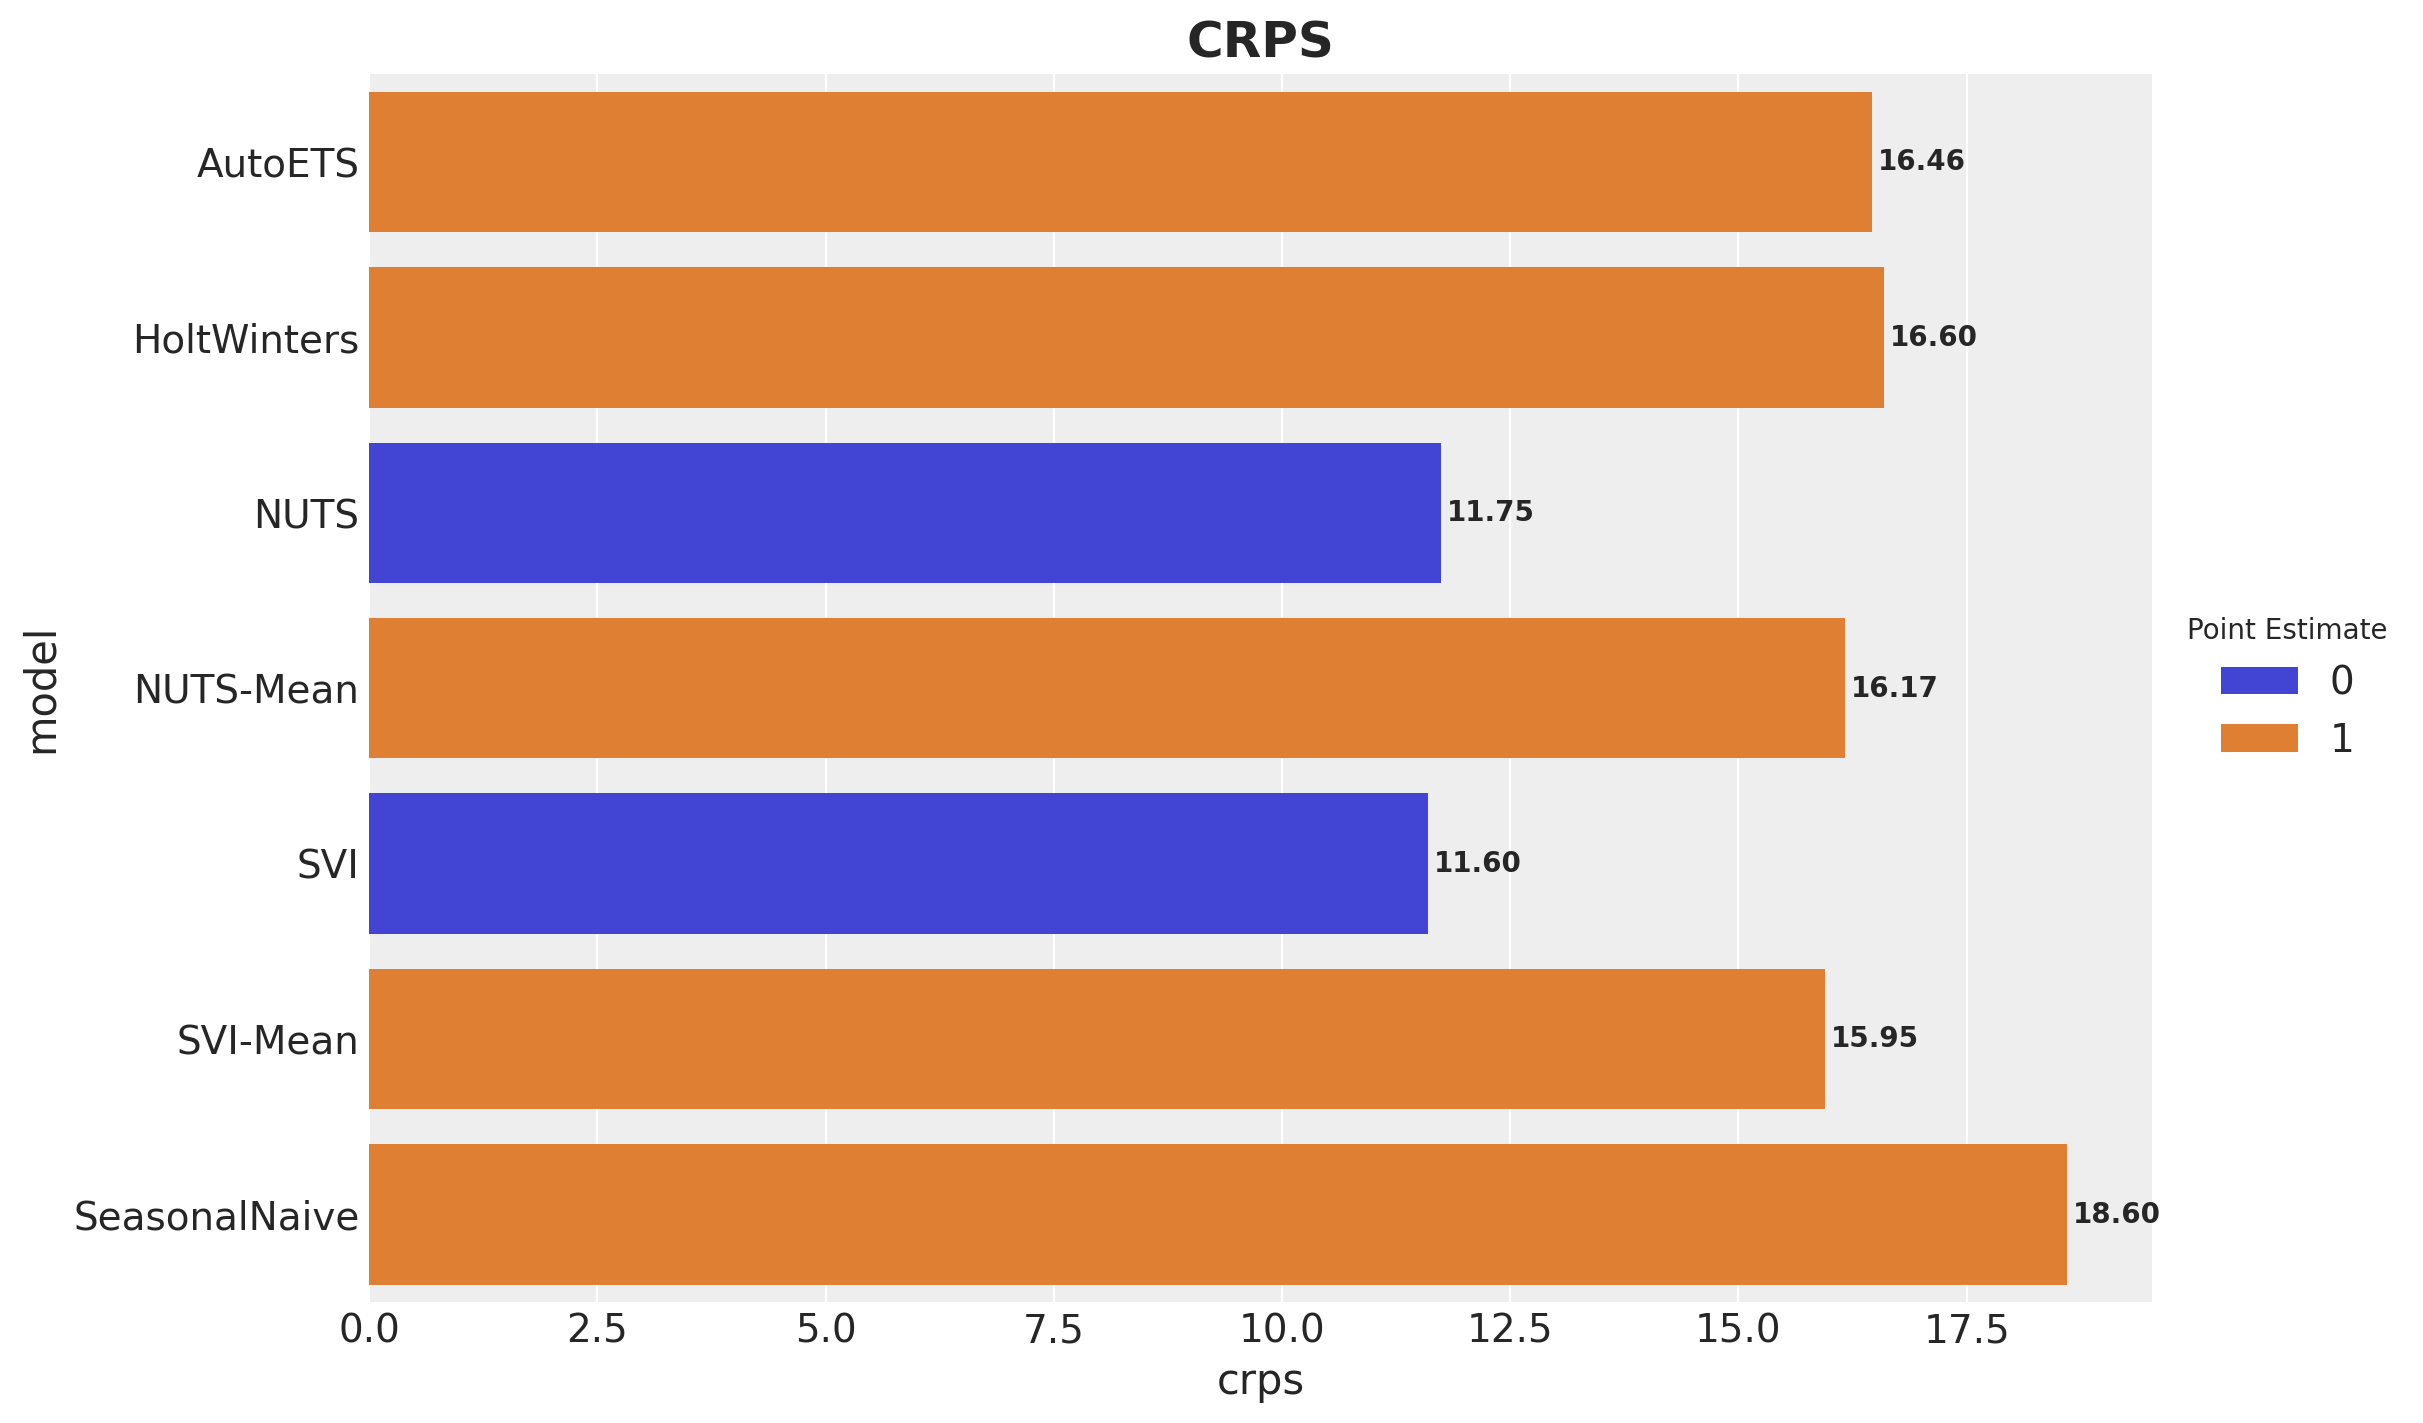
\includegraphics[width=0.95\linewidth]{hierarchical_exponential_smoothing_69_0.png}
\caption{Hierarchical exponential smoothing on Australian tourism data. Posterior predictive medians and credible intervals are shown for several regions sharing population-level innovation variances. Smaller regions borrow strength from larger ones without losing their distinctive seasonality.}
\label{fig:hier}
\end{figure}

What the substrate enables that off-the-shelf libraries typically do not is the freedom to mix hierarchy levels. The model can be made hierarchical in level dynamics but not in seasonality, or hierarchical across regions and across product categories at the same time. Each new hierarchical structure is a few additional \texttt{plate} statements rather than a change in framework.

\subsection{Intermittent demand under availability constraints}
\label{sec:avail}

Retail demand often contains long runs of zeros. Some of those zeros reflect genuine absence of demand; others reflect stockouts where demand existed but could not be observed because the product was not on the shelf. Classical intermittent-demand methods such as Croston's method \citep{croston1972forecasting} and the Teunter-Syntetos-Babai (TSB) variant \citep{teunter2011intermittent} model demand as a product of an interval (or probability) component and a size component, but they do not distinguish supply-driven zeros from demand-driven zeros. Recent work has noted the importance of separating these mechanisms \citep{svetunkov_zeros, pedregal2024tobit}.

The availability-aware TSB model \citep{orduz_availability_tsb} modifies the TSB transition to fold a known availability indicator into the probability update. When the product is observed unavailable, the demand-probability state is preserved rather than updated downward, so a long stockout does not corrupt the model into believing demand has vanished. The modification is mathematically small but operationally important: the resulting forecasts of latent demand are unbiased under common stockout regimes. Figure~\ref{fig:avail} shows the availability mask and the resulting forecast for a representative product.

\begin{figure}[!htbp]
\centering
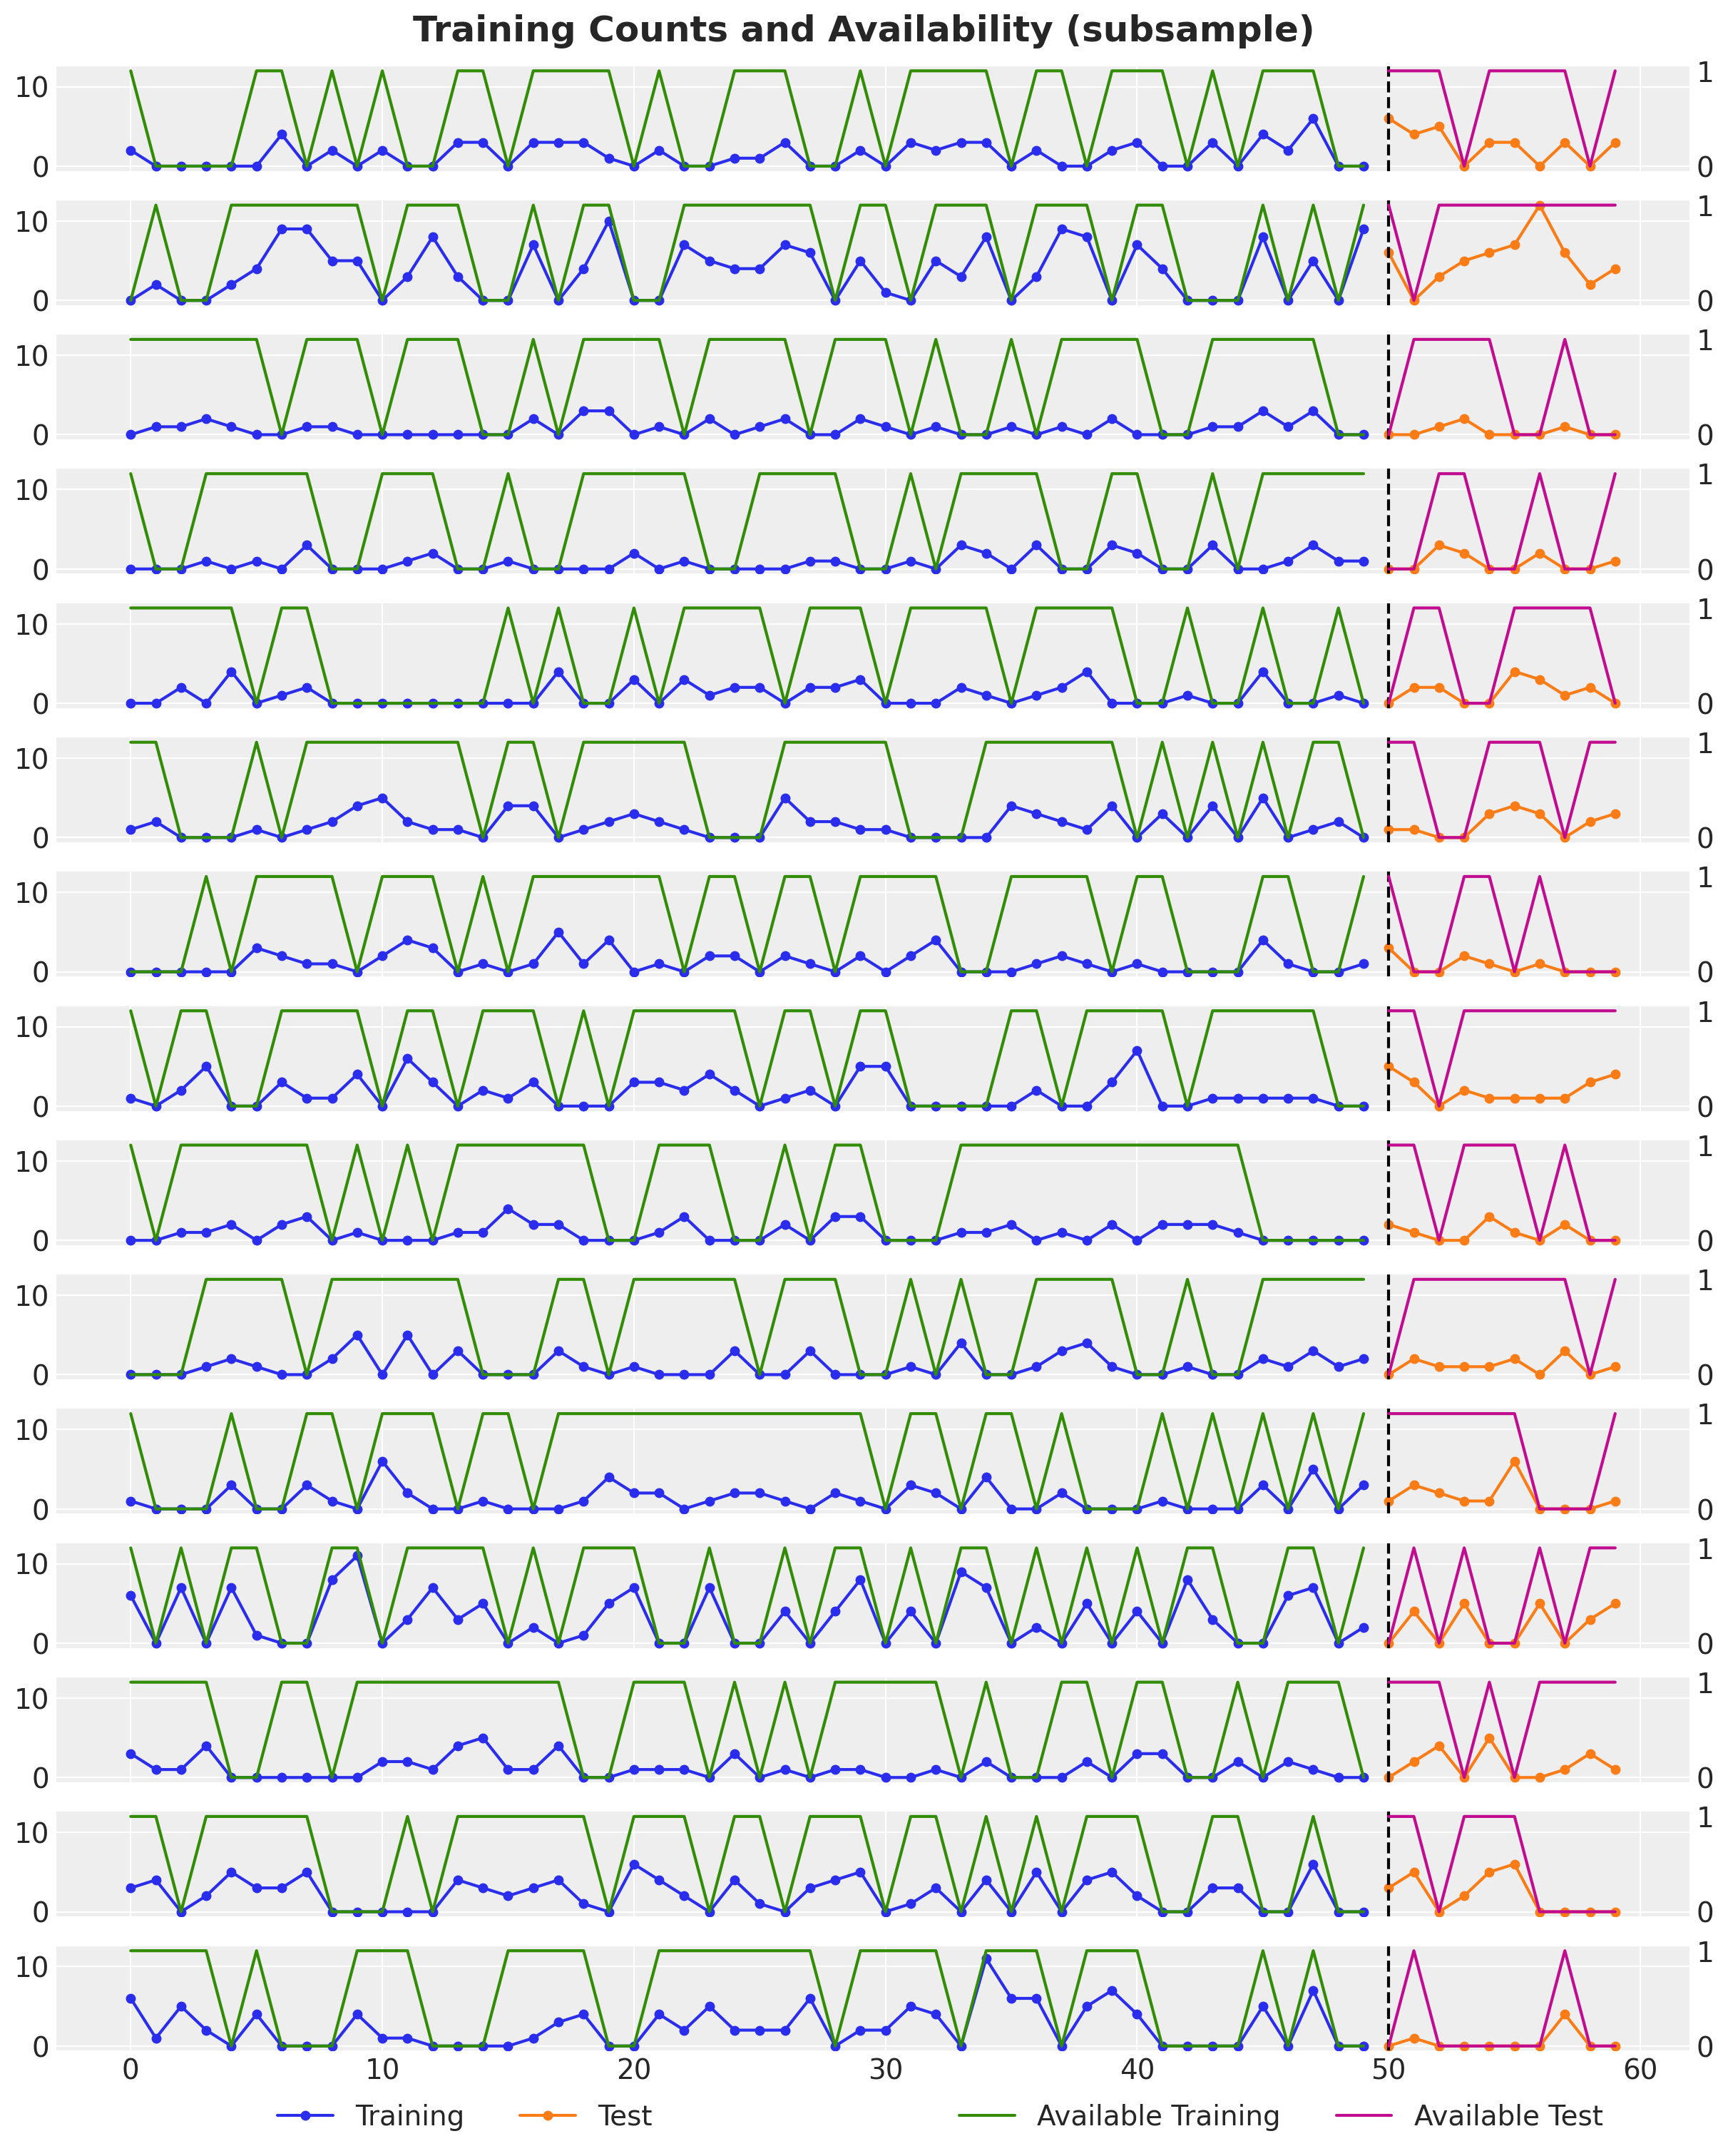
\includegraphics[width=0.62\linewidth]{availability_tsb_12_0.png}\\[0.5ex]
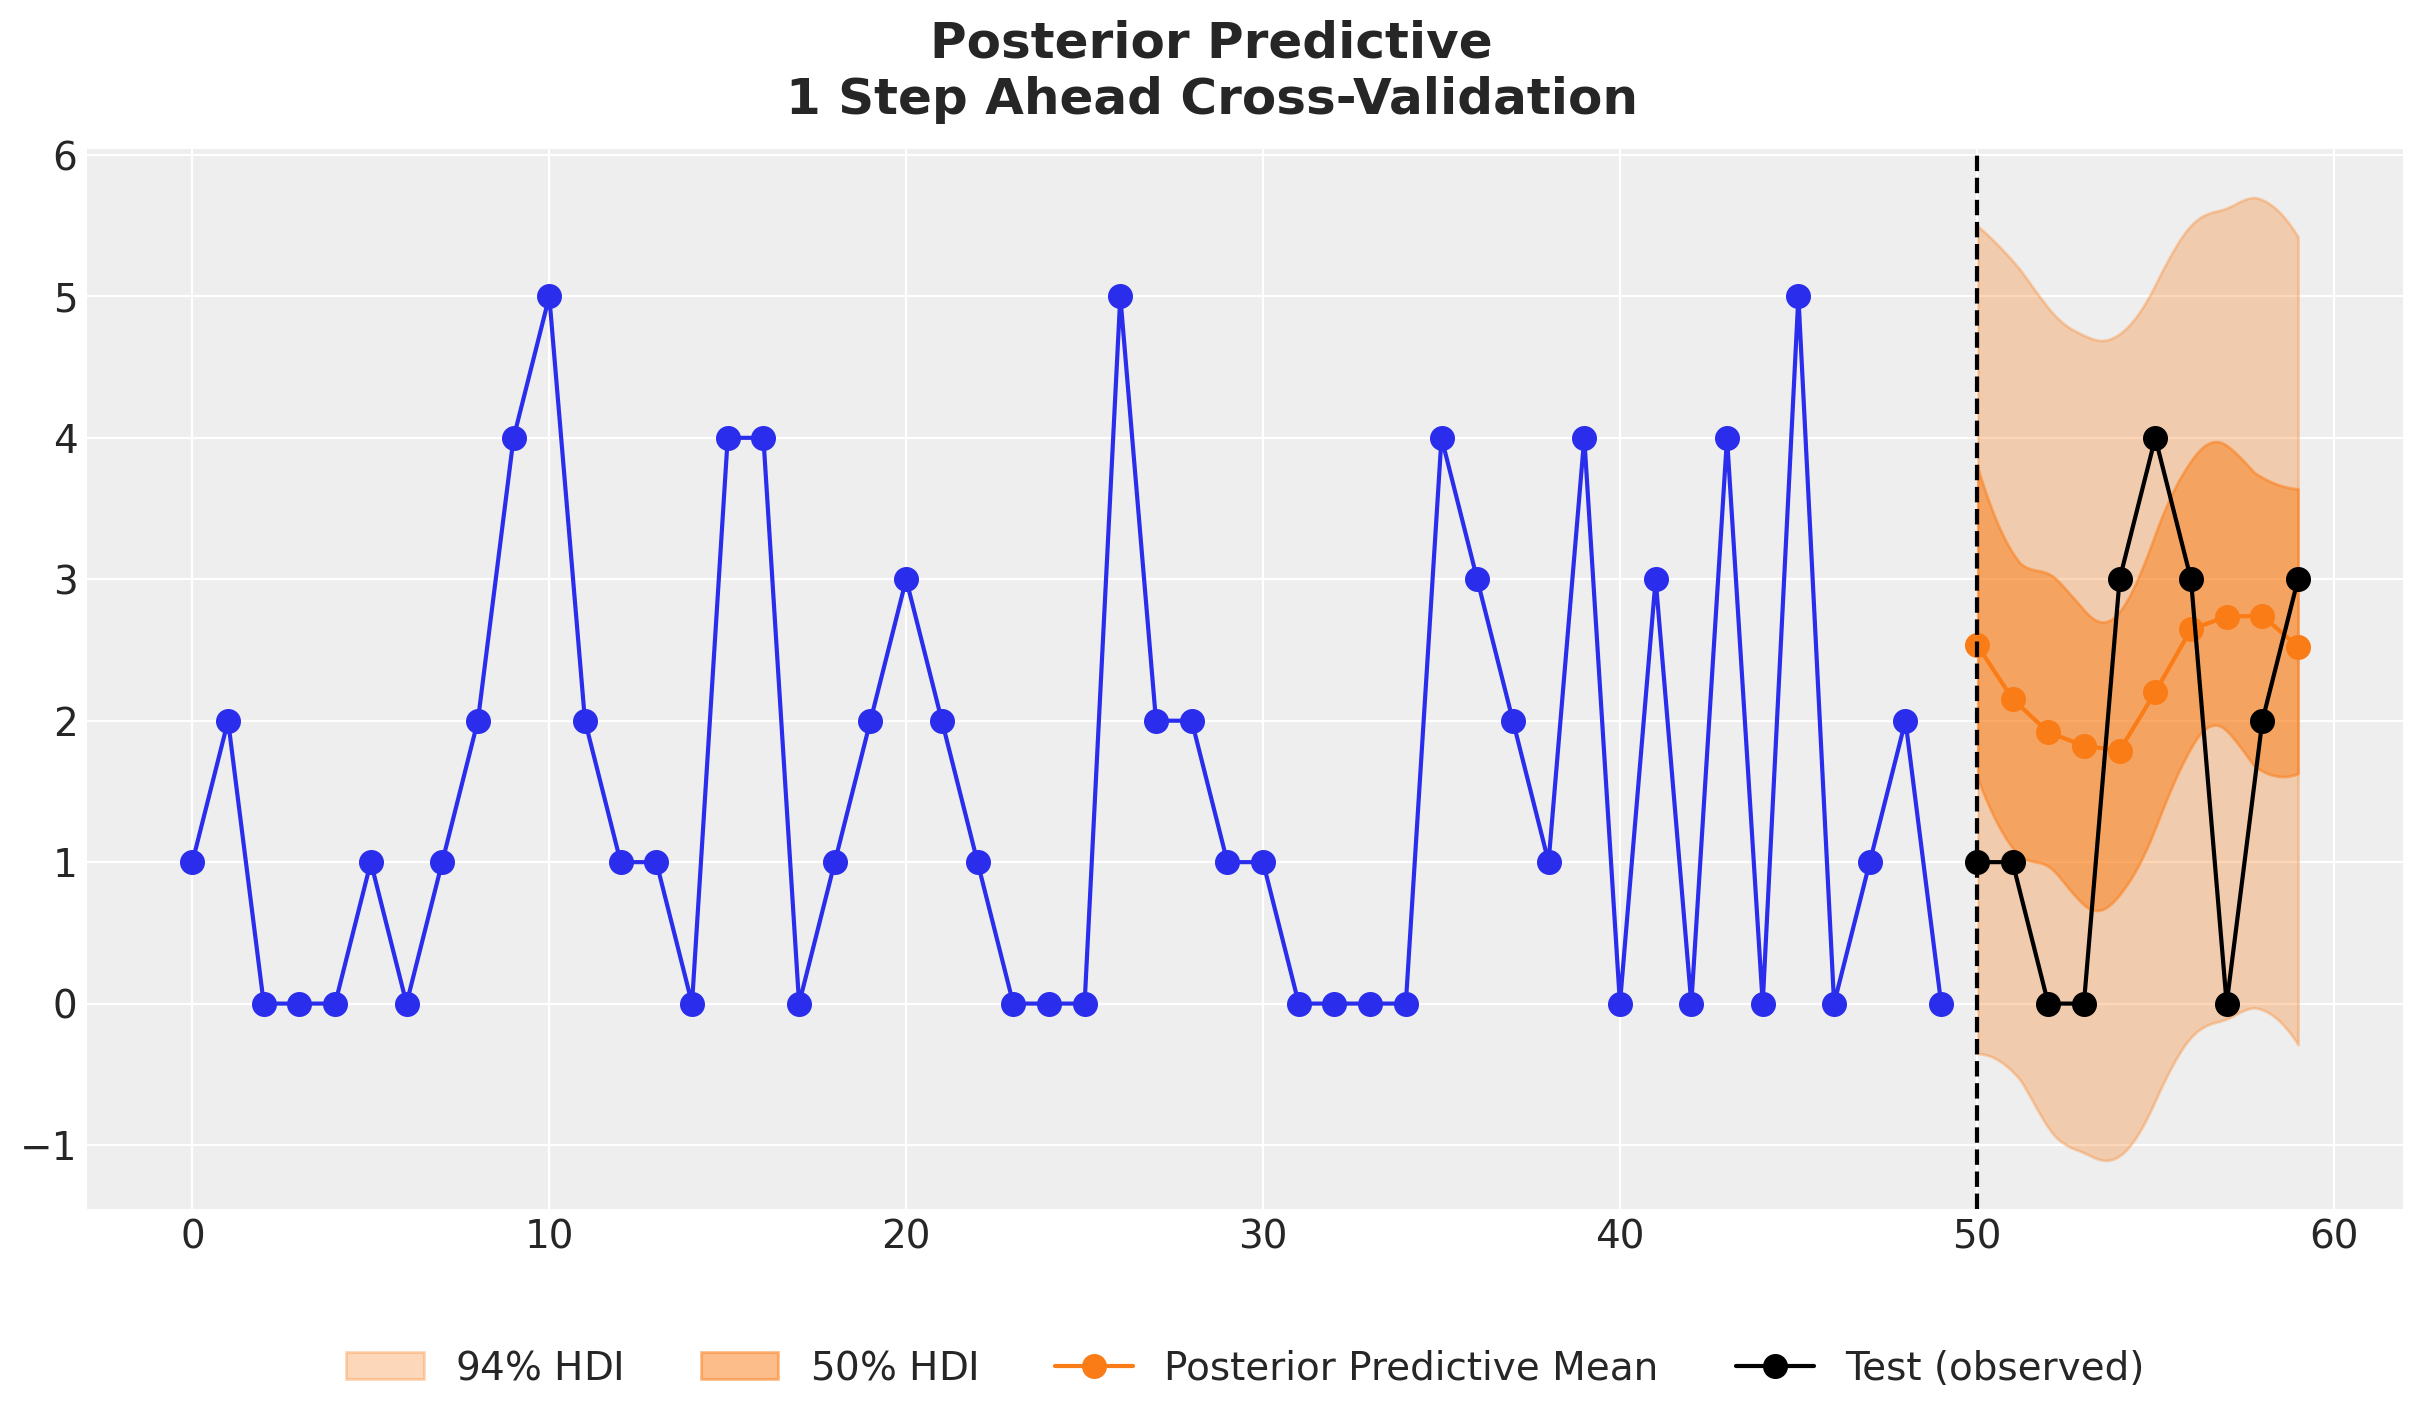
\includegraphics[width=0.62\linewidth]{availability_tsb_38_0.png}
\caption{Top: an observed sales series with the corresponding availability mask. Long runs of zeros coincide with periods when the item was unavailable. Bottom: posterior predictive forecast from the availability-aware TSB model. The model recovers latent demand from intermittent and partially censored observations.}
\label{fig:avail}
\end{figure}

This case study is, in our view, the clearest example of why a composable substrate has a role to play alongside pre-packaged libraries. The availability-aware TSB transition is not in any standard library because it is a one-off model for a particular operational reality. Implementing it in NumPyro requires only writing the modified transition function inside a \texttt{scan}; nothing else about the model changes. The substrate enables a model that does not exist as an off-the-shelf option.

\subsection{Censored demand under stockouts}
\label{sec:cens}

A complementary view of the same operational reality is censored regression. Rather than treating stockouts as a state-update modifier, censored models treat observed sales during a stockout as a lower bound on true demand. The likelihood for an observation $y_t$ that is censored at capacity $c_t$ is the survival function of the assumed demand distribution evaluated at $c_t$; for uncensored observations it is the ordinary density. This insight, applied carefully to demand forecasting, is the subject of recent practitioner-led work \citep{caron_censored} and is implemented end-to-end in a NumPyro worked example \citep{orduz_censoring, orduz_demand}.

In NumPyro the censored likelihood is expressed by combining a standard distribution for the latent demand process with a conditional log-probability that switches between density and survival depending on the censoring indicator. The mechanics are uneventful: a few lines of code inside a \texttt{scan} step. The consequence for the forecast is large. Figure~\ref{fig:cens} contrasts the posterior demand estimate under a naive model with that of the censored model.

\begin{figure}[!htbp]
\centering
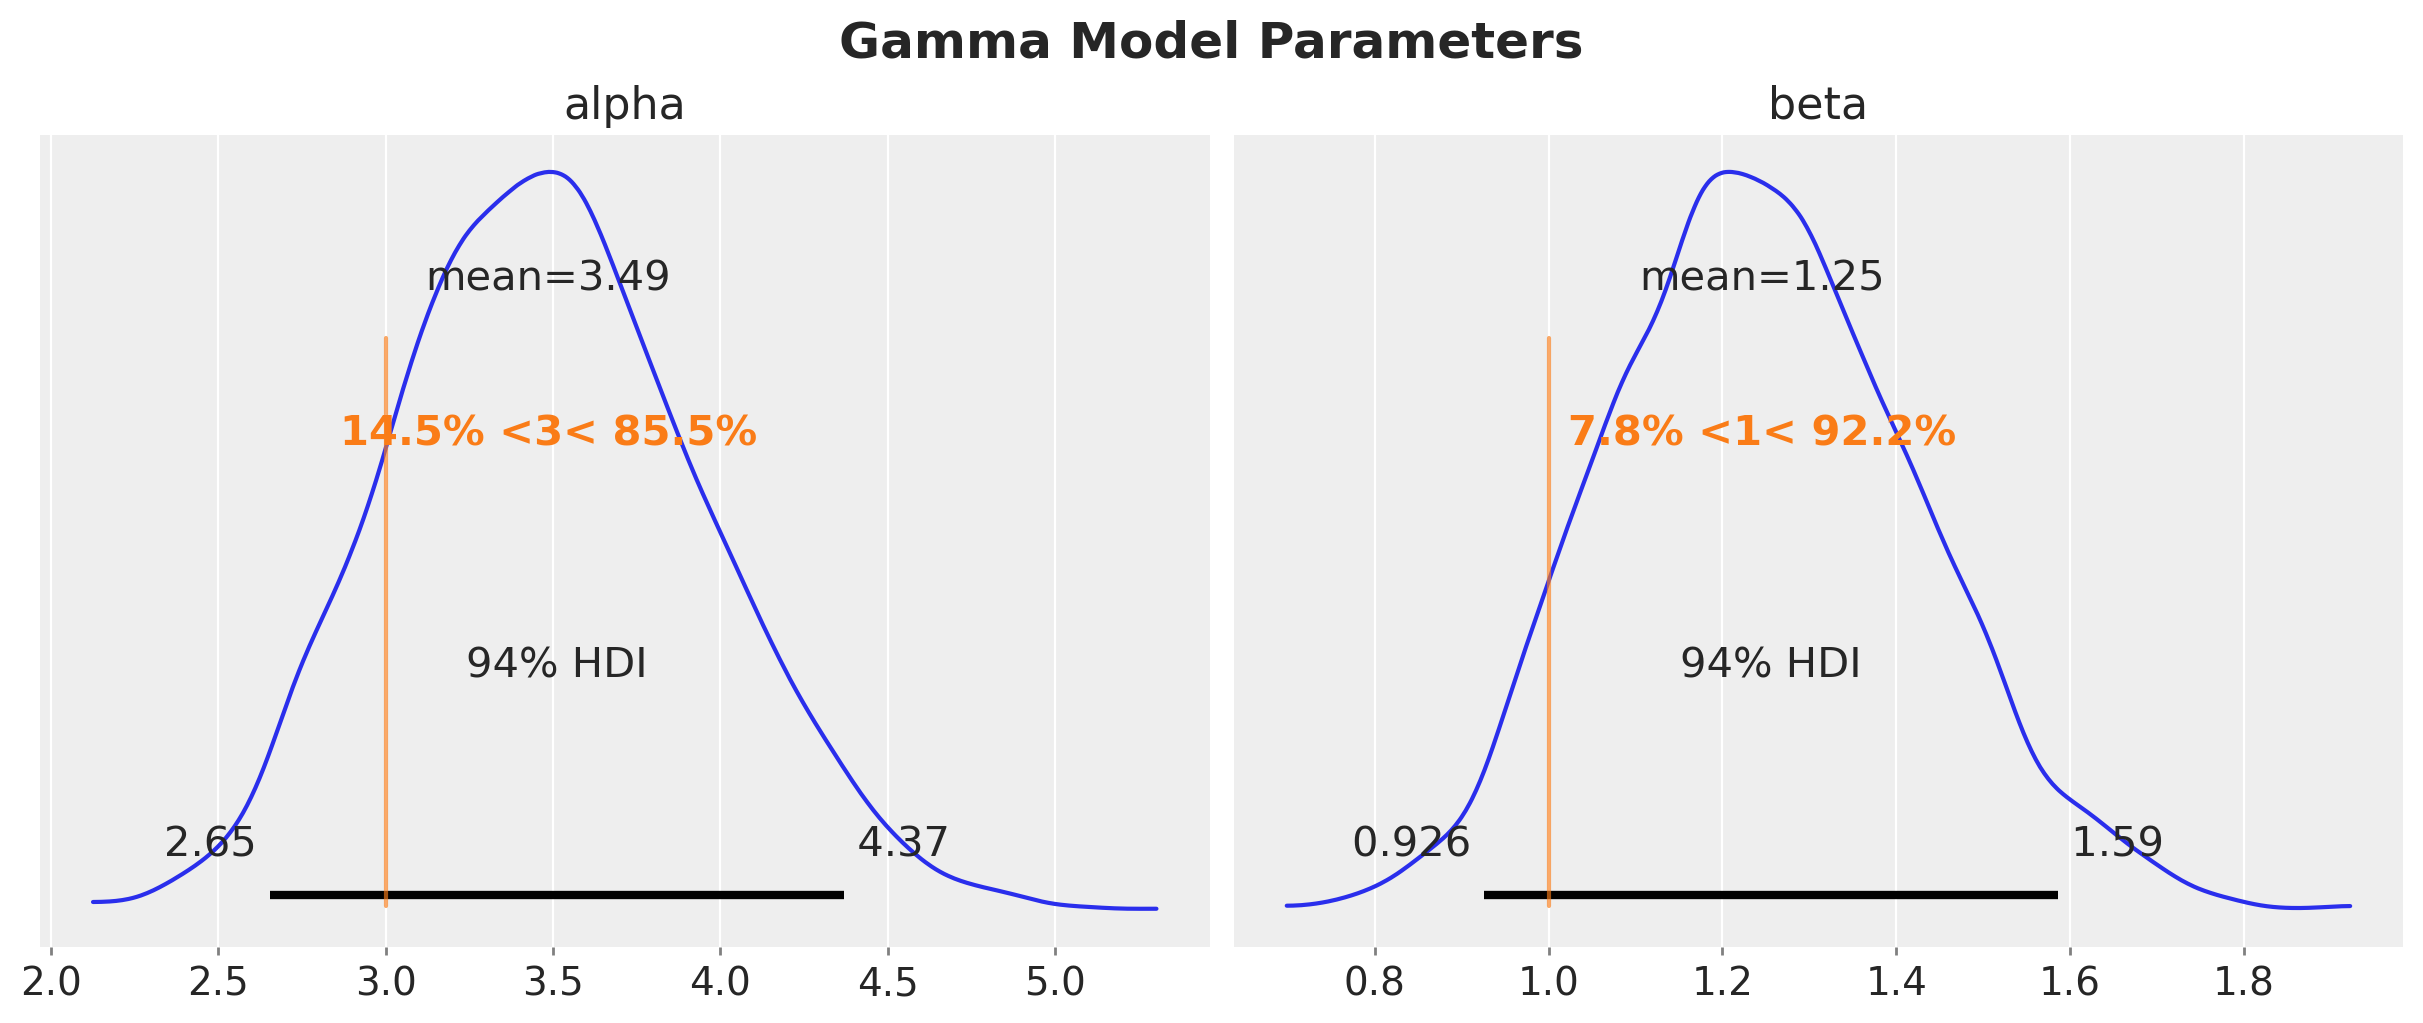
\includegraphics[width=0.65\linewidth]{censoring_12_0.png}\\[1ex]
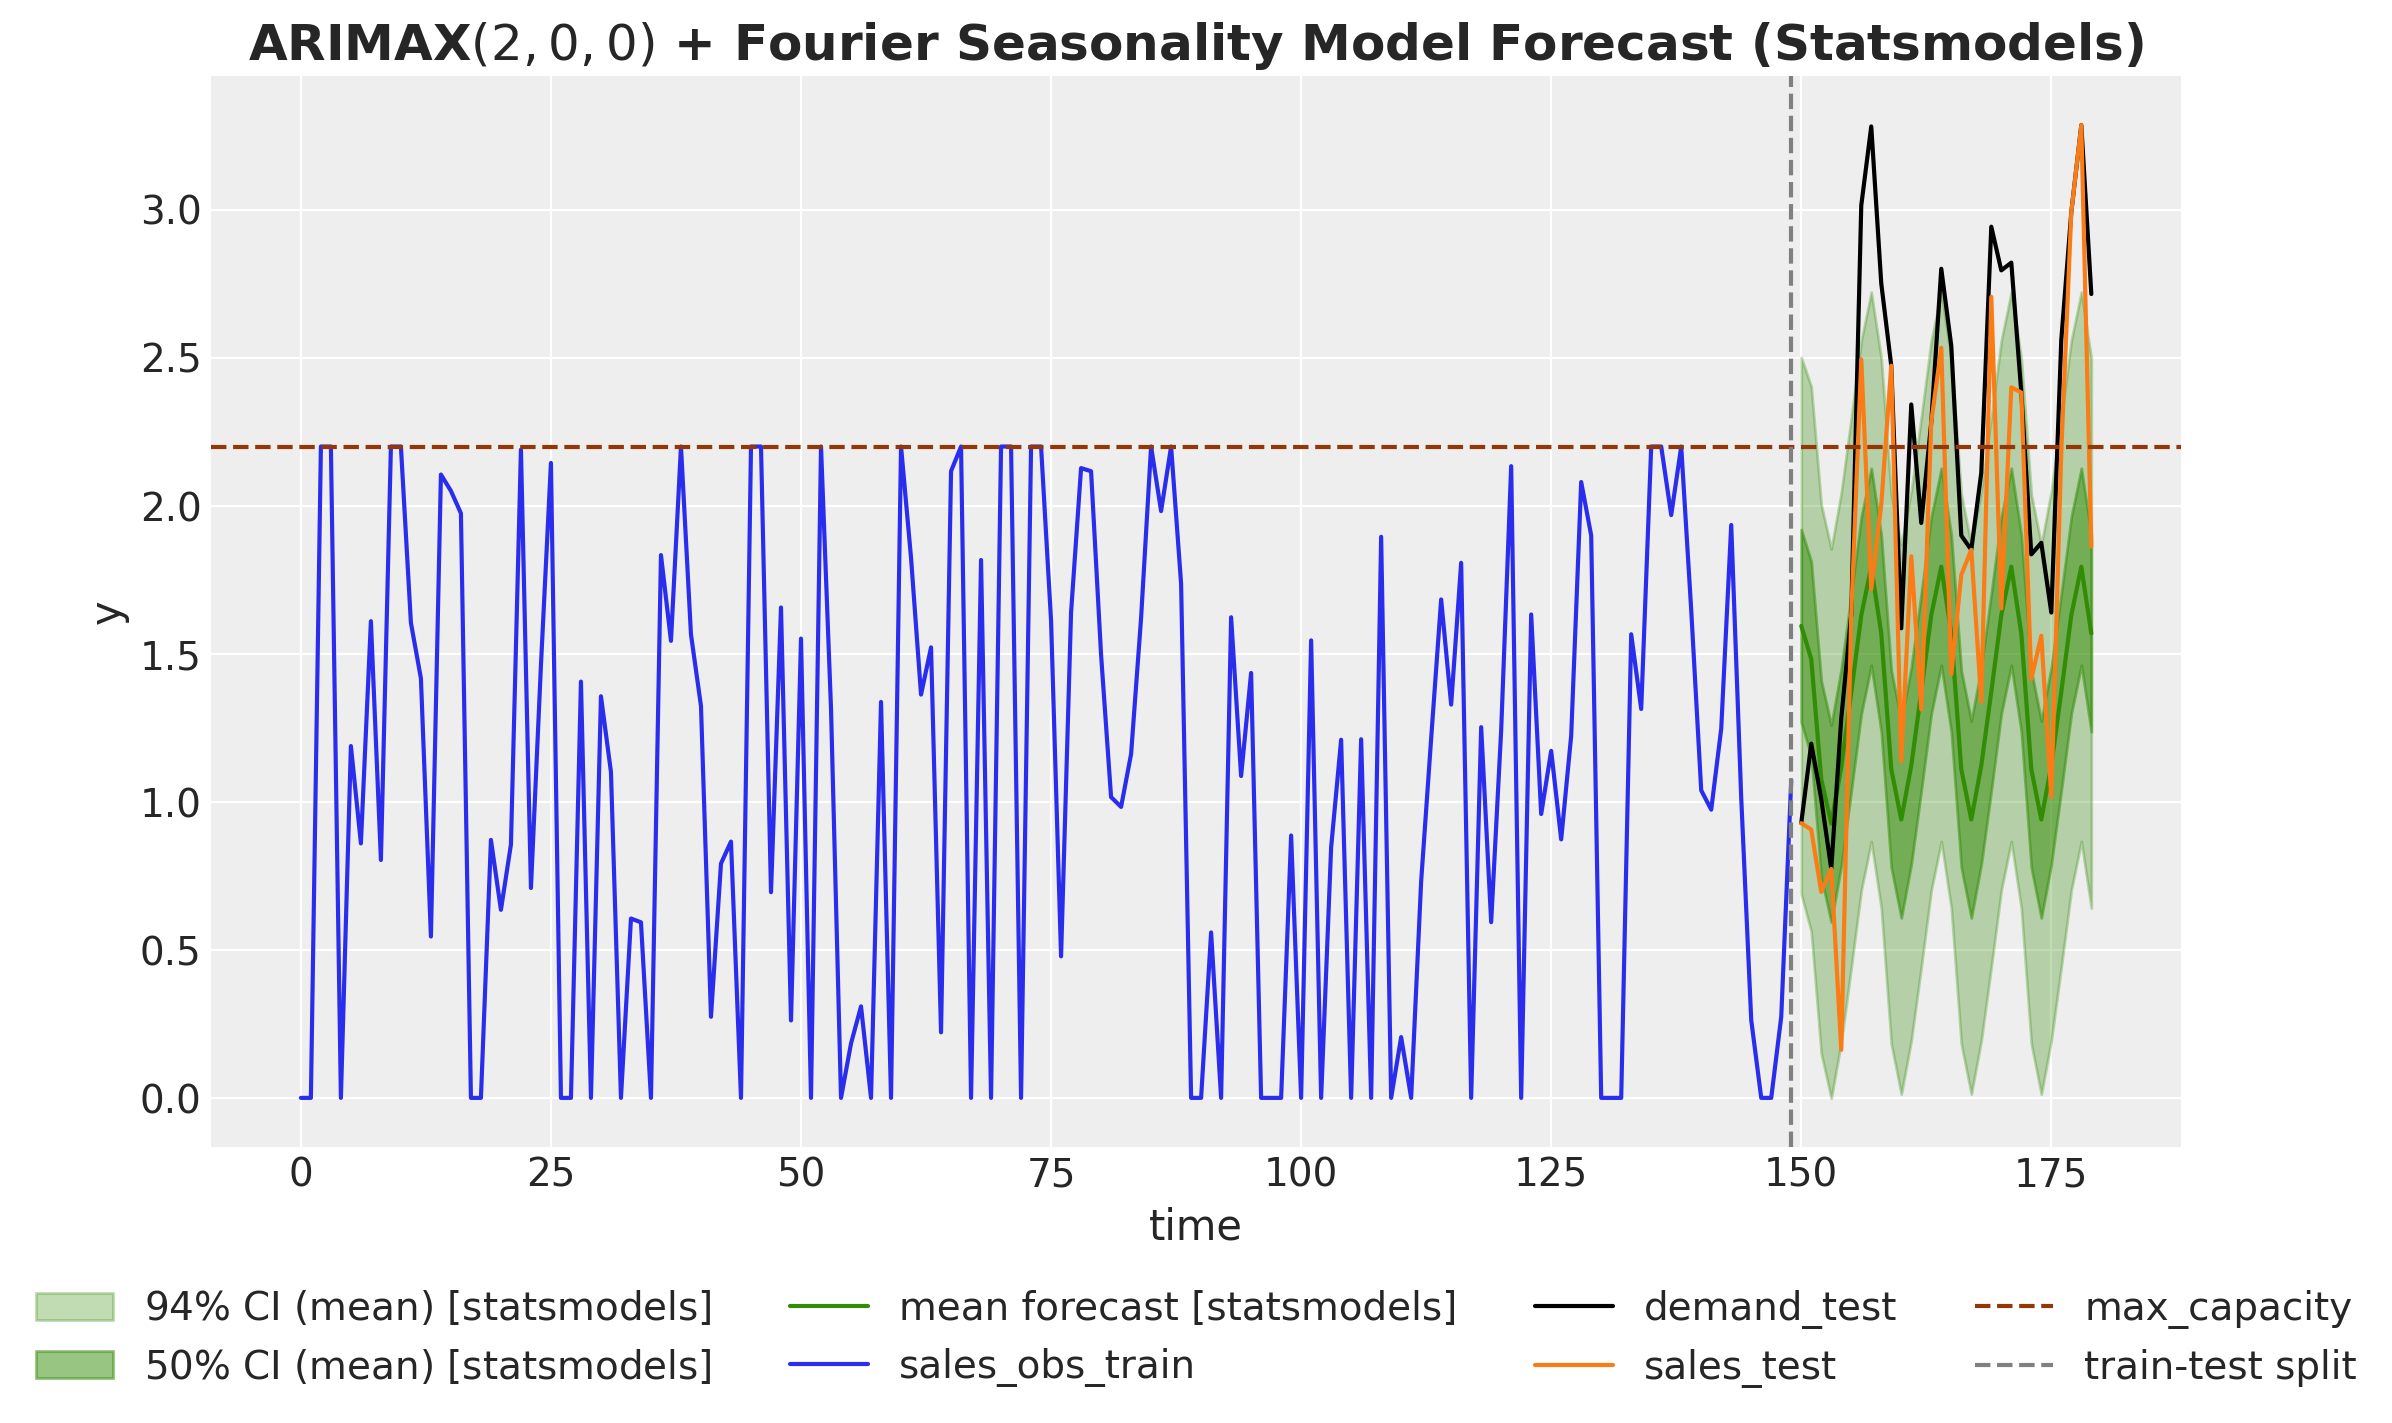
\includegraphics[width=0.65\linewidth]{demand_25_0.png}
\caption{Top: synthetic demand with a hard capacity ceiling and the associated censoring events. Bottom: latent demand recovered by the censored model. A model that ignores censoring underestimates the right tail; the censored model recovers it.}
\label{fig:cens}
\end{figure}

Censored likelihoods appear in many forecasting domains beyond retail, including grid-capacity-constrained energy and revenue-management contexts where bookings are limited by inventory. The substrate handles all of them in the same way: write the appropriate log-probability and let inference take care of the rest.

\subsection{Bayesian vector autoregression}
\label{sec:var}

Multivariate forecasting introduces the additional challenge of modeling cross-series dependence. Vector autoregressive (VAR) models specify a linear map from the lagged joint state to the current joint state, with innovations drawn from a multivariate distribution. Frequentist VARs are well established in econometrics, but a Bayesian treatment offers two practical benefits: regularization of the autoregressive coefficient matrices via informative priors, and full posterior distributions over impulse-response functions rather than point estimates.

Our worked example \citep{orduz_var} fits a Bayesian VAR with NUTS using LKJ priors on the correlation structure of the innovation covariance and weakly informative priors on the autoregressive coefficients. Compared with a packaged VAR routine, what the substrate adds is direct control over this prior structure: shrinkage on the coefficient matrices and an LKJ prior on the innovation correlations are a few lines rather than a fork of someone else's estimator, and they yield full posteriors over derived quantities instead of point estimates. There is a trade-off worth stating: for a dense linear-Gaussian state-space model like this one, marginalizing the latent states with a Kalman filter can be more efficient than sampling them through \texttt{scan}, and JAX state-space libraries such as \texttt{dynamax} \citep{dynamax} compose here too when that route is preferred. The recursive evaluation is, again, a single \texttt{scan} over the multivariate state. Once posterior samples are available, impulse-response functions are computed inside another \texttt{vmap} over posterior draws and shock sources, which yields uncertainty bands rather than point trajectories. Figure~\ref{fig:var} reports the resulting impulse-response functions for a small economic system.

\begin{figure}[h]
\centering
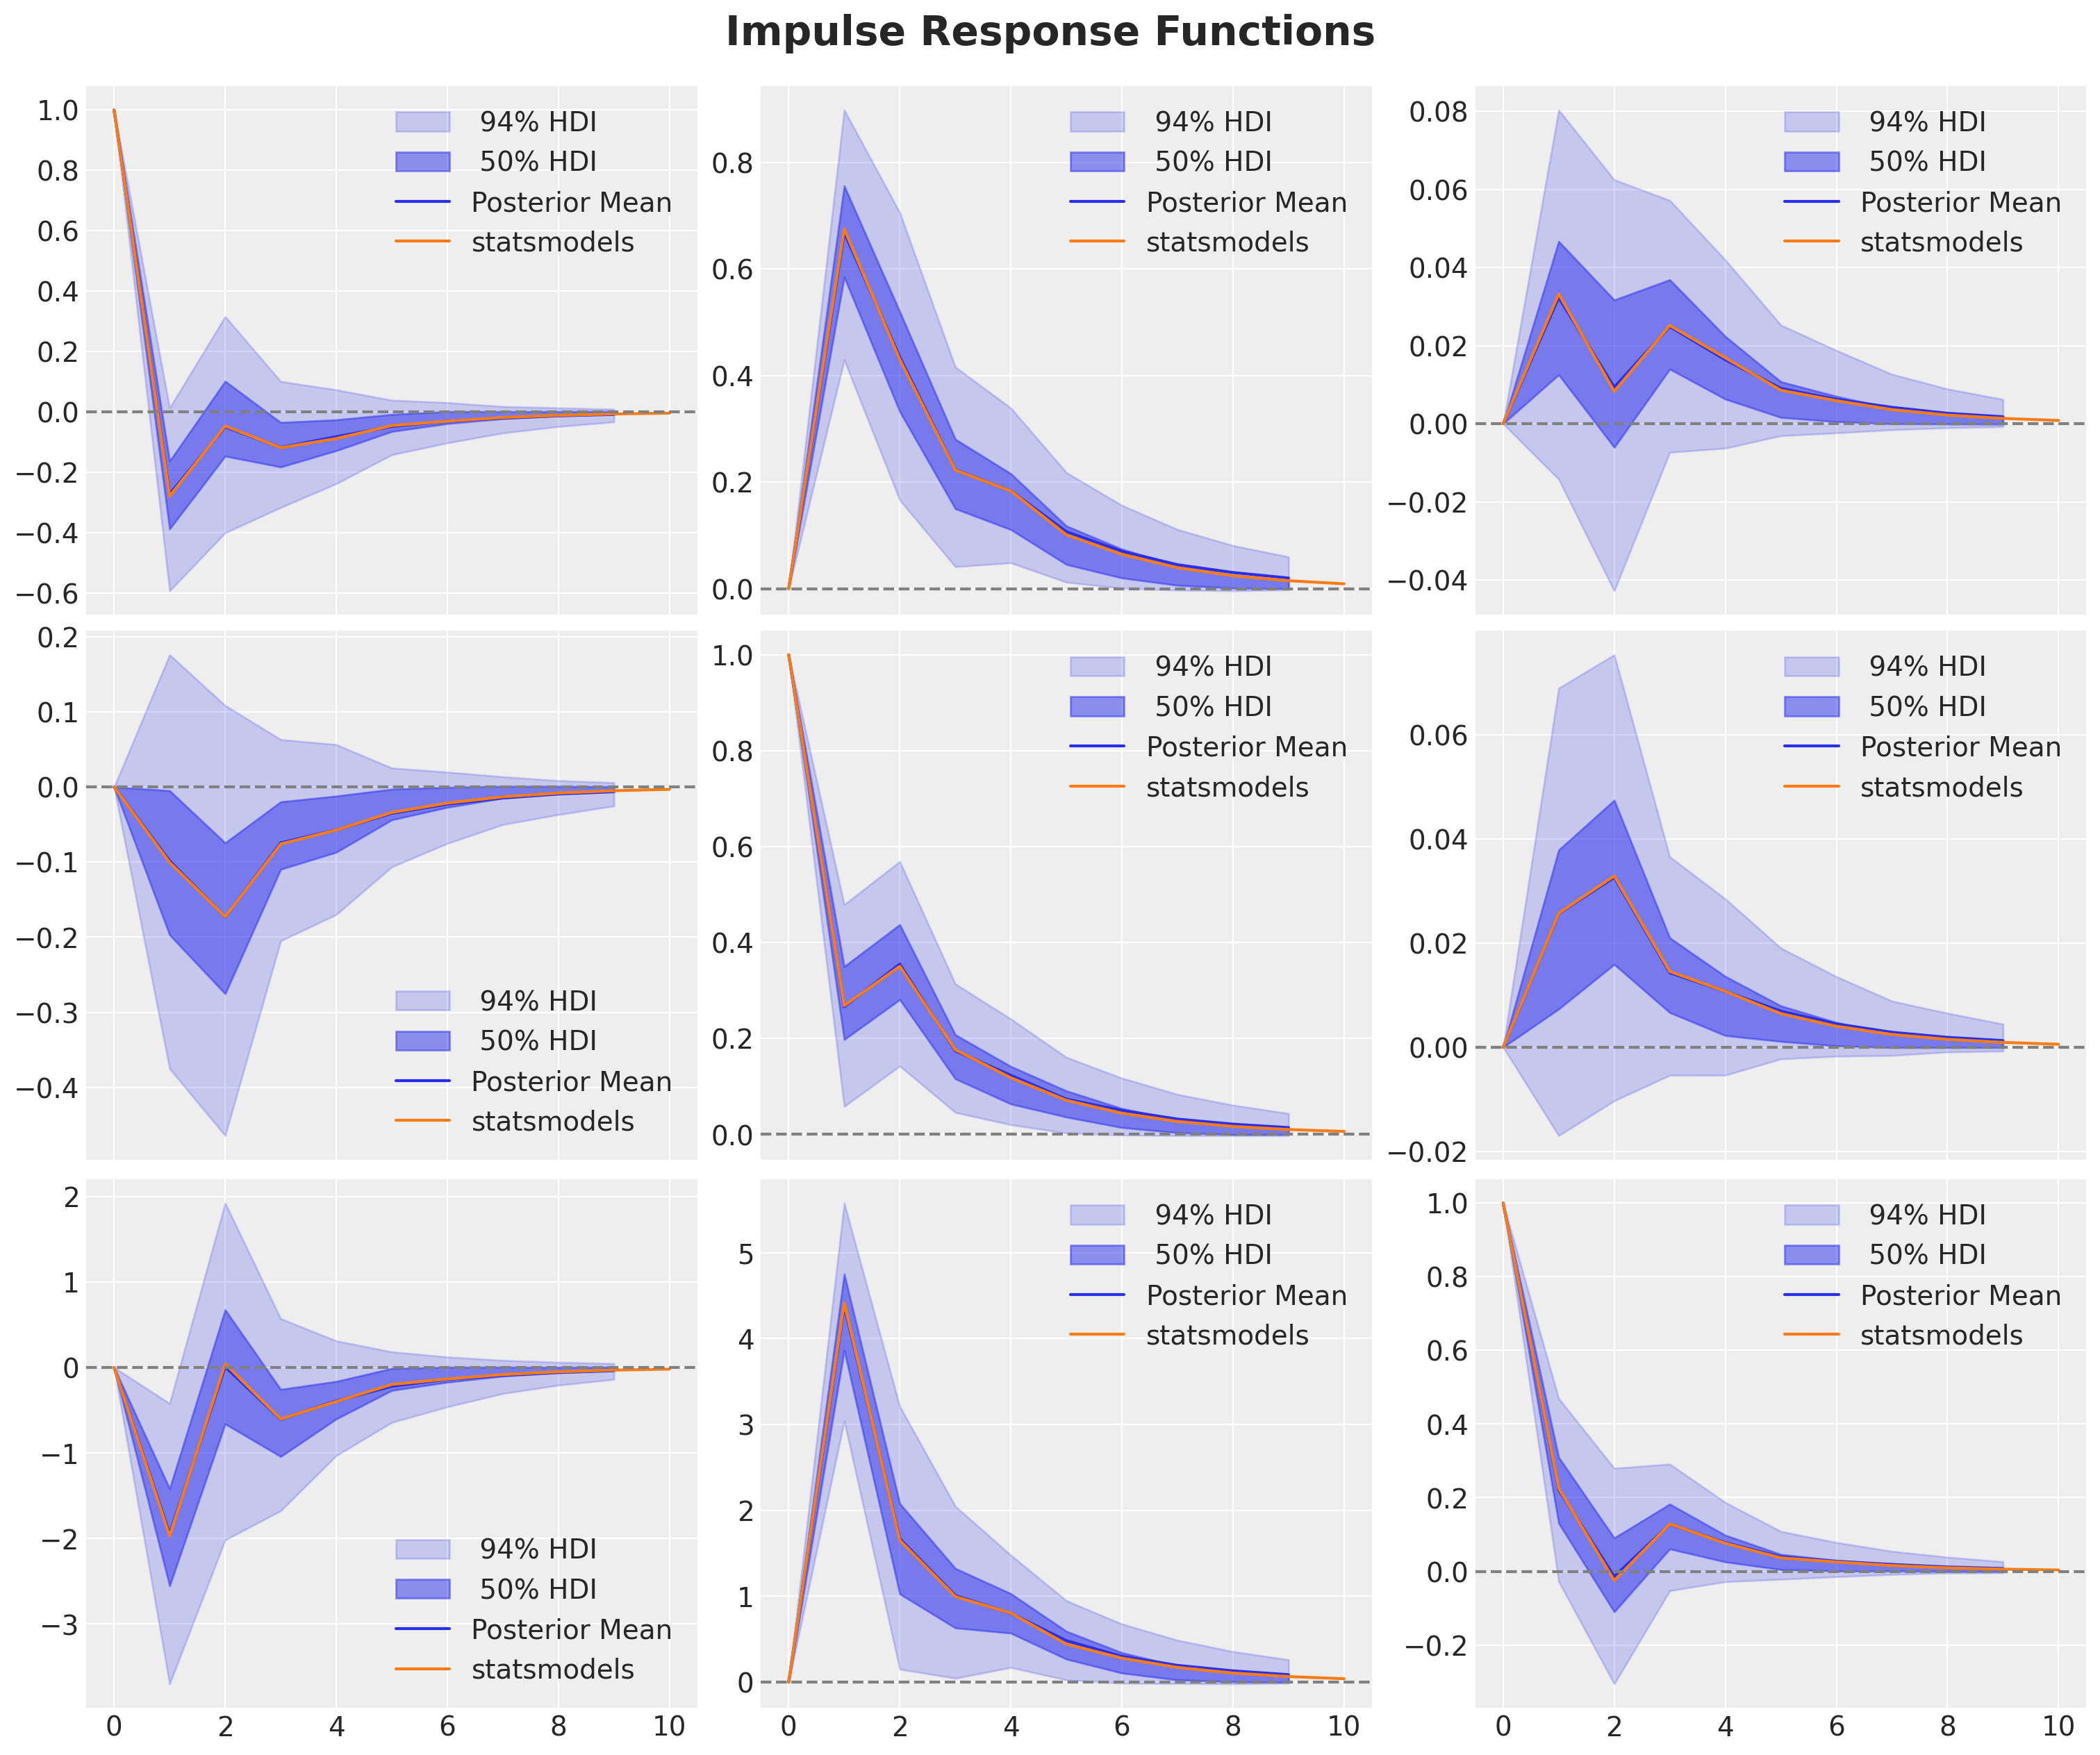
\includegraphics[width=0.95\linewidth]{var_irf.png}
\caption{Posterior impulse-response functions from a Bayesian VAR(2) model fit with NUTS in NumPyro. Each panel shows the response of one variable to a unit shock in another, with shaded credible intervals reflecting parameter uncertainty.}
\label{fig:var}
\end{figure}

A practical observation here is that the JAX ecosystem makes the downstream analysis as cheap as the model itself. Computing impulse-response functions across thousands of posterior samples is a vectorized JAX operation rather than a Python loop. This collapses a multi-hour postprocessing pipeline in some traditional environments into a sub-second batched call.

\subsection{Gaussian processes via Hilbert-space approximation}
\label{sec:hsgp}

Smooth covariate effects, long-period seasonality, and slowly varying trend components are all well captured by Gaussian processes. The computational difficulty of GPs is well known: exact inference scales cubically in the number of observations, which rules them out for typical forecasting series of any length. Hilbert-space approximate Gaussian processes (HSGP), introduced by \citet{riutort2022practical}, reformulate the GP as a finite-dimensional linear-in-coefficients model whose basis is derived from the eigenfunctions of the Laplacian on a bounded domain. The result is a GP that fits and predicts in linear time and that composes cleanly with other model components.

Our electricity demand example \citep{orduz_electricity} uses an HSGP for the temperature-response curve combined with a level-and-seasonality state-space backbone. We apply the HSGP to the temperature covariate here for exposition, but nothing restricts it to covariate effects: the same basis construction can represent a smooth trend or a long-period seasonal component, and these uses compose additively within one model. Because the HSGP is a linear model in its basis coefficients, it slots into the larger forecasting model with no special inference treatment. Figure~\ref{fig:hsgp} shows the resulting hourly demand forecast with credible bands that respect the nonlinear temperature dependence.

\begin{figure}[h]
\centering
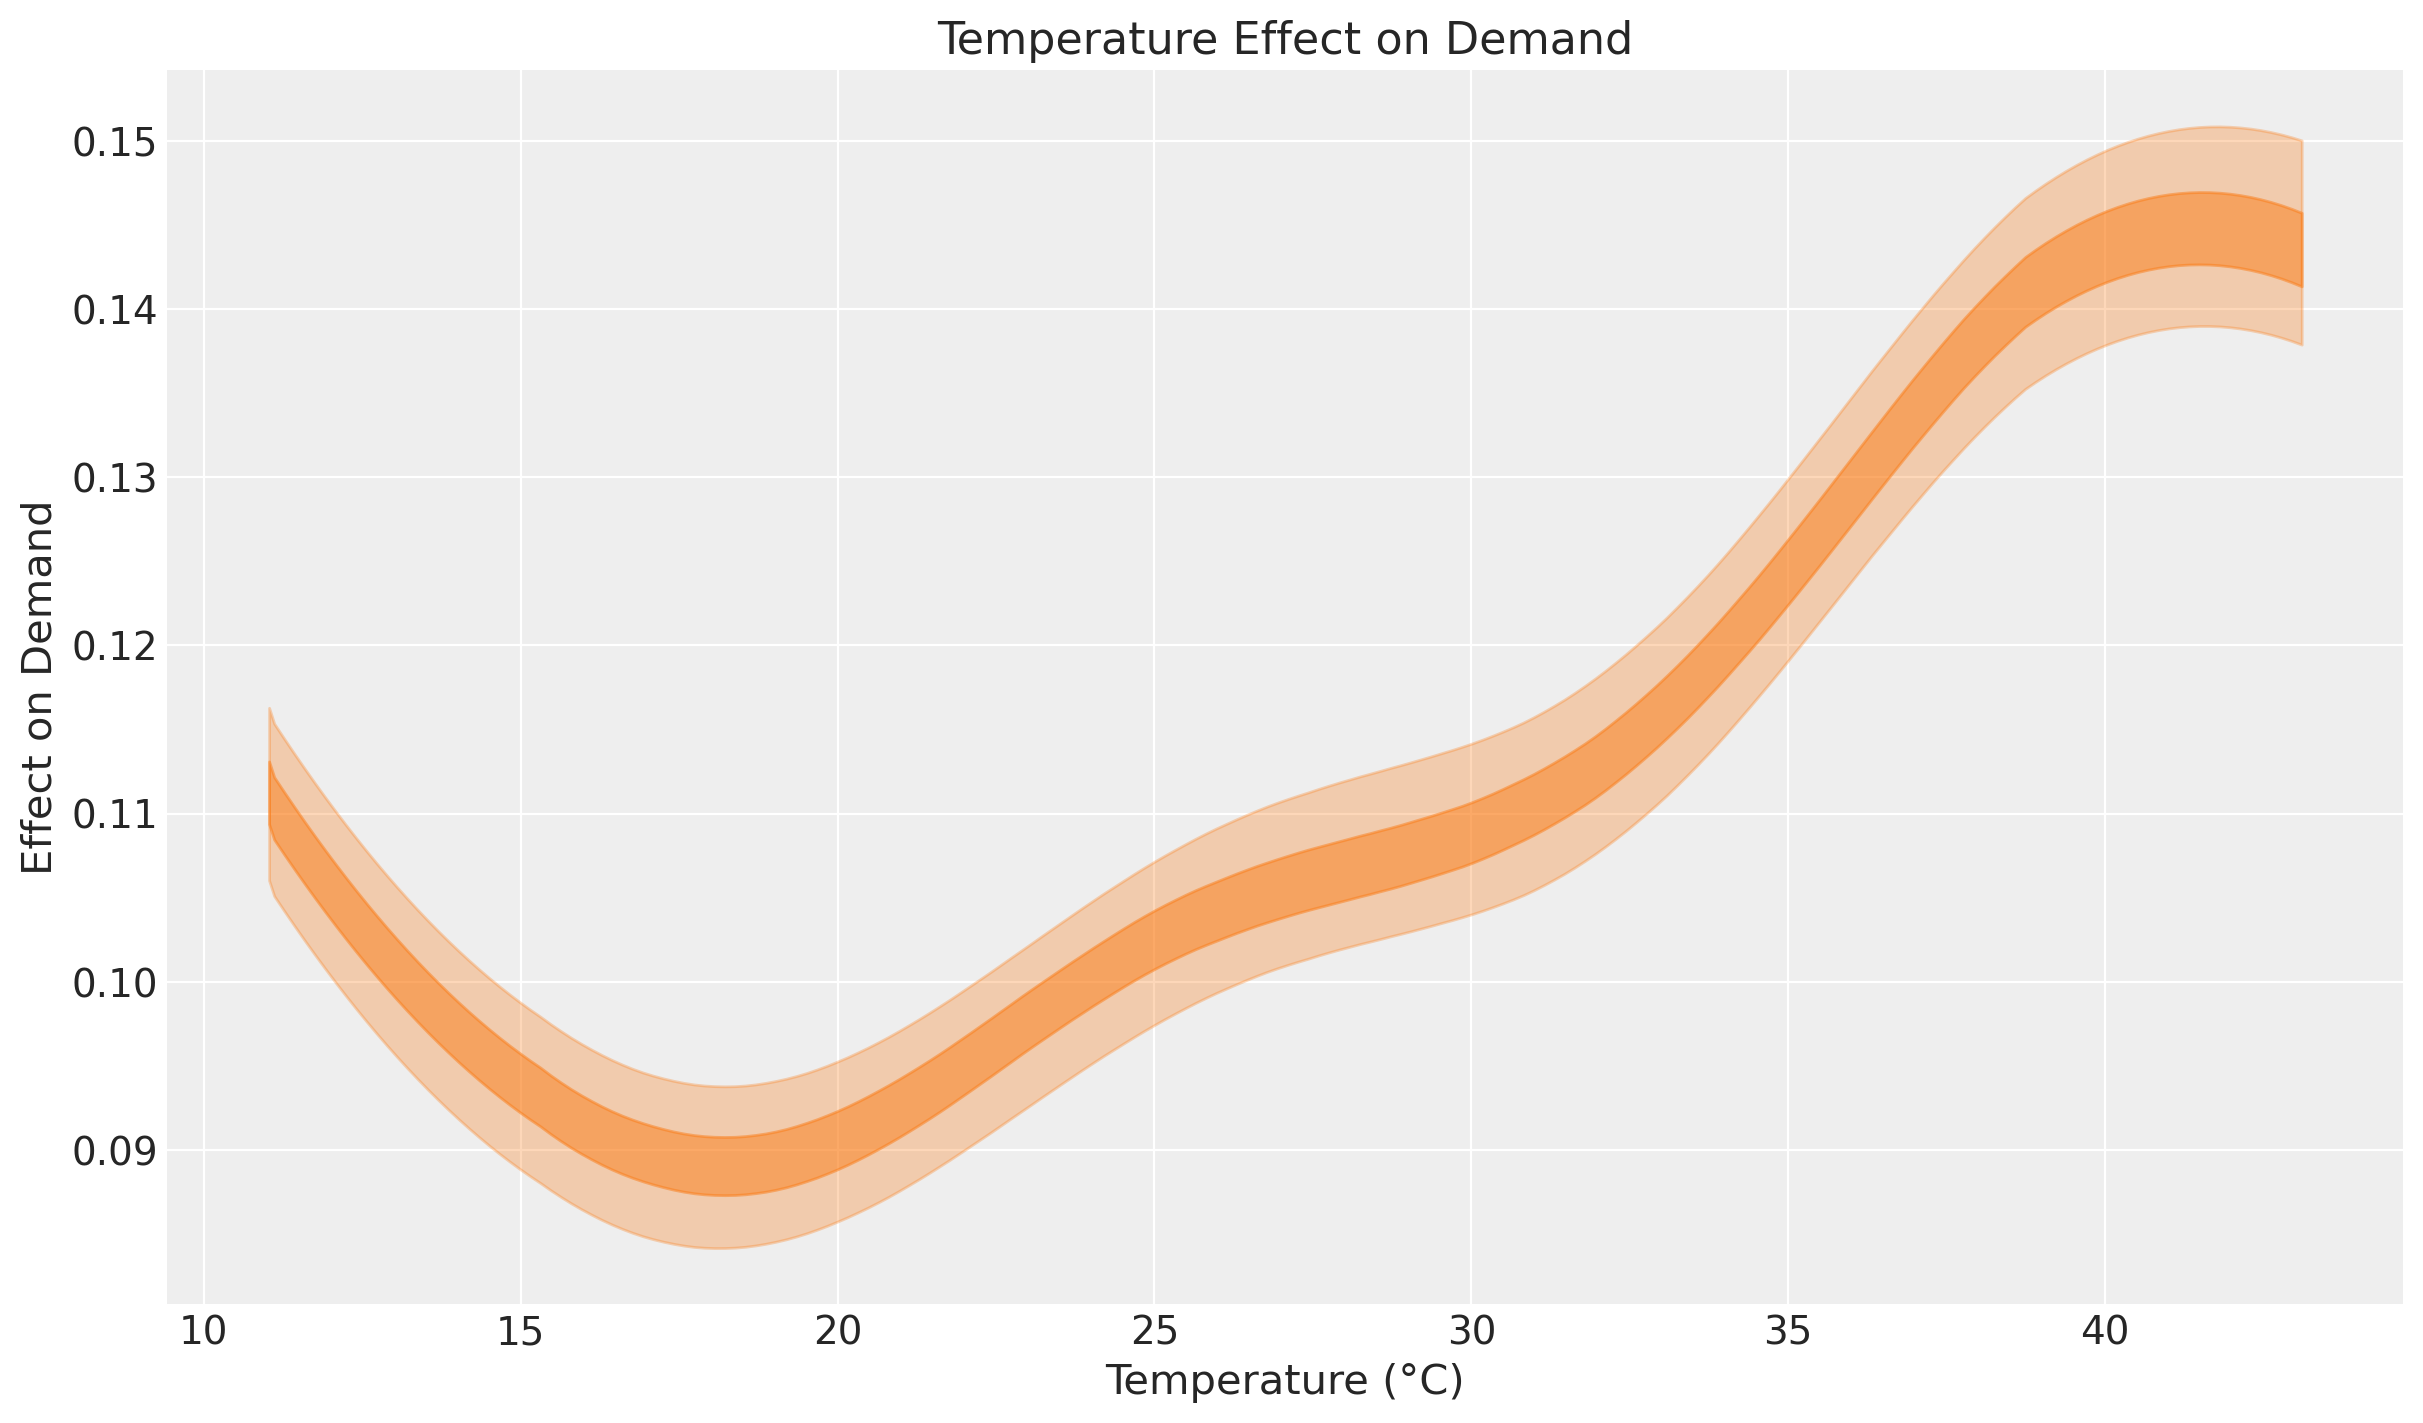
\includegraphics[width=0.95\linewidth]{electricity_forecast_46_0.png}
\caption{Electricity demand forecast combining a state-space level-and-seasonality backbone with an HSGP for the temperature-response curve. The credible interval reflects both the dynamic-state uncertainty and the nonlinear covariate uncertainty.}
\label{fig:hsgp}
\end{figure}

The story we draw from this case study is again about composability. The HSGP is a model component, not a separate library. It composes with the rest of the forecasting model through the same primitives we have already discussed: a linear contribution inside a \texttt{scan} step.

The same composability is what lets a practitioner express structured covariate effects that an off-the-shelf forecaster does not expose. A common need is an event or holiday feature whose temporal shape is shared across a panel of series but whose magnitude varies from one series to the next. This is a few lines: a shared basis with partially pooled, non-centered loadings.

\begin{lstlisting}
import jax.numpy as jnp
import numpyro
import numpyro.distributions as dist

def event_basis(X, n_nodes):  # X: (time, cov, basis)
    n_time, n_cov, n_basis = X.shape
    beta_loc = numpyro.sample("beta_loc", dist.Normal(0.0, 0.3))
    beta_scale = numpyro.sample("beta_scale", dist.HalfNormal(0.3))
    beta_raw = numpyro.sample("beta_raw", dist.Normal(0, 1).expand([n_cov, n_basis]))
    beta = beta_loc + beta_scale * beta_raw  # shape per cov

    load_loc = numpyro.sample("load_loc", dist.Normal(0, 0.3).expand([n_cov]))
    load_scale = numpyro.sample("load_scale", dist.HalfNormal(0.3).expand([n_cov]))
    load_raw = numpyro.sample("load_raw", dist.Normal(0, 1).expand([n_nodes, n_cov]))
    loadings = load_loc + load_scale * load_raw  # per series

    shape = jnp.einsum("tcb,cb->tc", X, beta)
    return jnp.einsum("tc,jc->tj", shape, loadings)  # effect
\end{lstlisting}

Expressing this kind of non-time-series structure, rather than passing a covariate into a black-box slot, is in our experience the single most useful affordance of a probabilistic substrate over a packaged forecaster.

\subsection{Calibration via additional likelihoods}
\label{sec:calib}

The final case study is conceptually the most distinctive. Forecasting practice frequently involves auxiliary information that is not naturally encoded as a prior but is naturally encoded as a noisy observation. A marketing analyst may have results from a lift test that estimate the incremental effect of a campaign. A grid operator may have a physical reference point for the temperature-response of demand at a specific hour. A pricing team may have expert anchor points for the price elasticity of a specific segment. Each of these is a piece of information about a latent quantity in the model.

The trick, popularized in the probabilistic-programming community by the Pyro DLM tutorial \citep{pyro_dlm_tutorial} and explored further in our electricity-forecast-with-priors example \citep{orduz_electricity_priors}, is to encode the auxiliary information as additional likelihood terms. A lift test estimate becomes an observed-with-noise version of a posterior contrast. An expert anchor becomes an observed-with-noise version of a model output at a specific input. The forecasting model jointly explains the historical series and the auxiliary observations under a single coherent posterior. Figure~\ref{fig:calib} shows how this calibration tightens the temperature-response curve in the electricity model.

\begin{figure}[h]
\centering
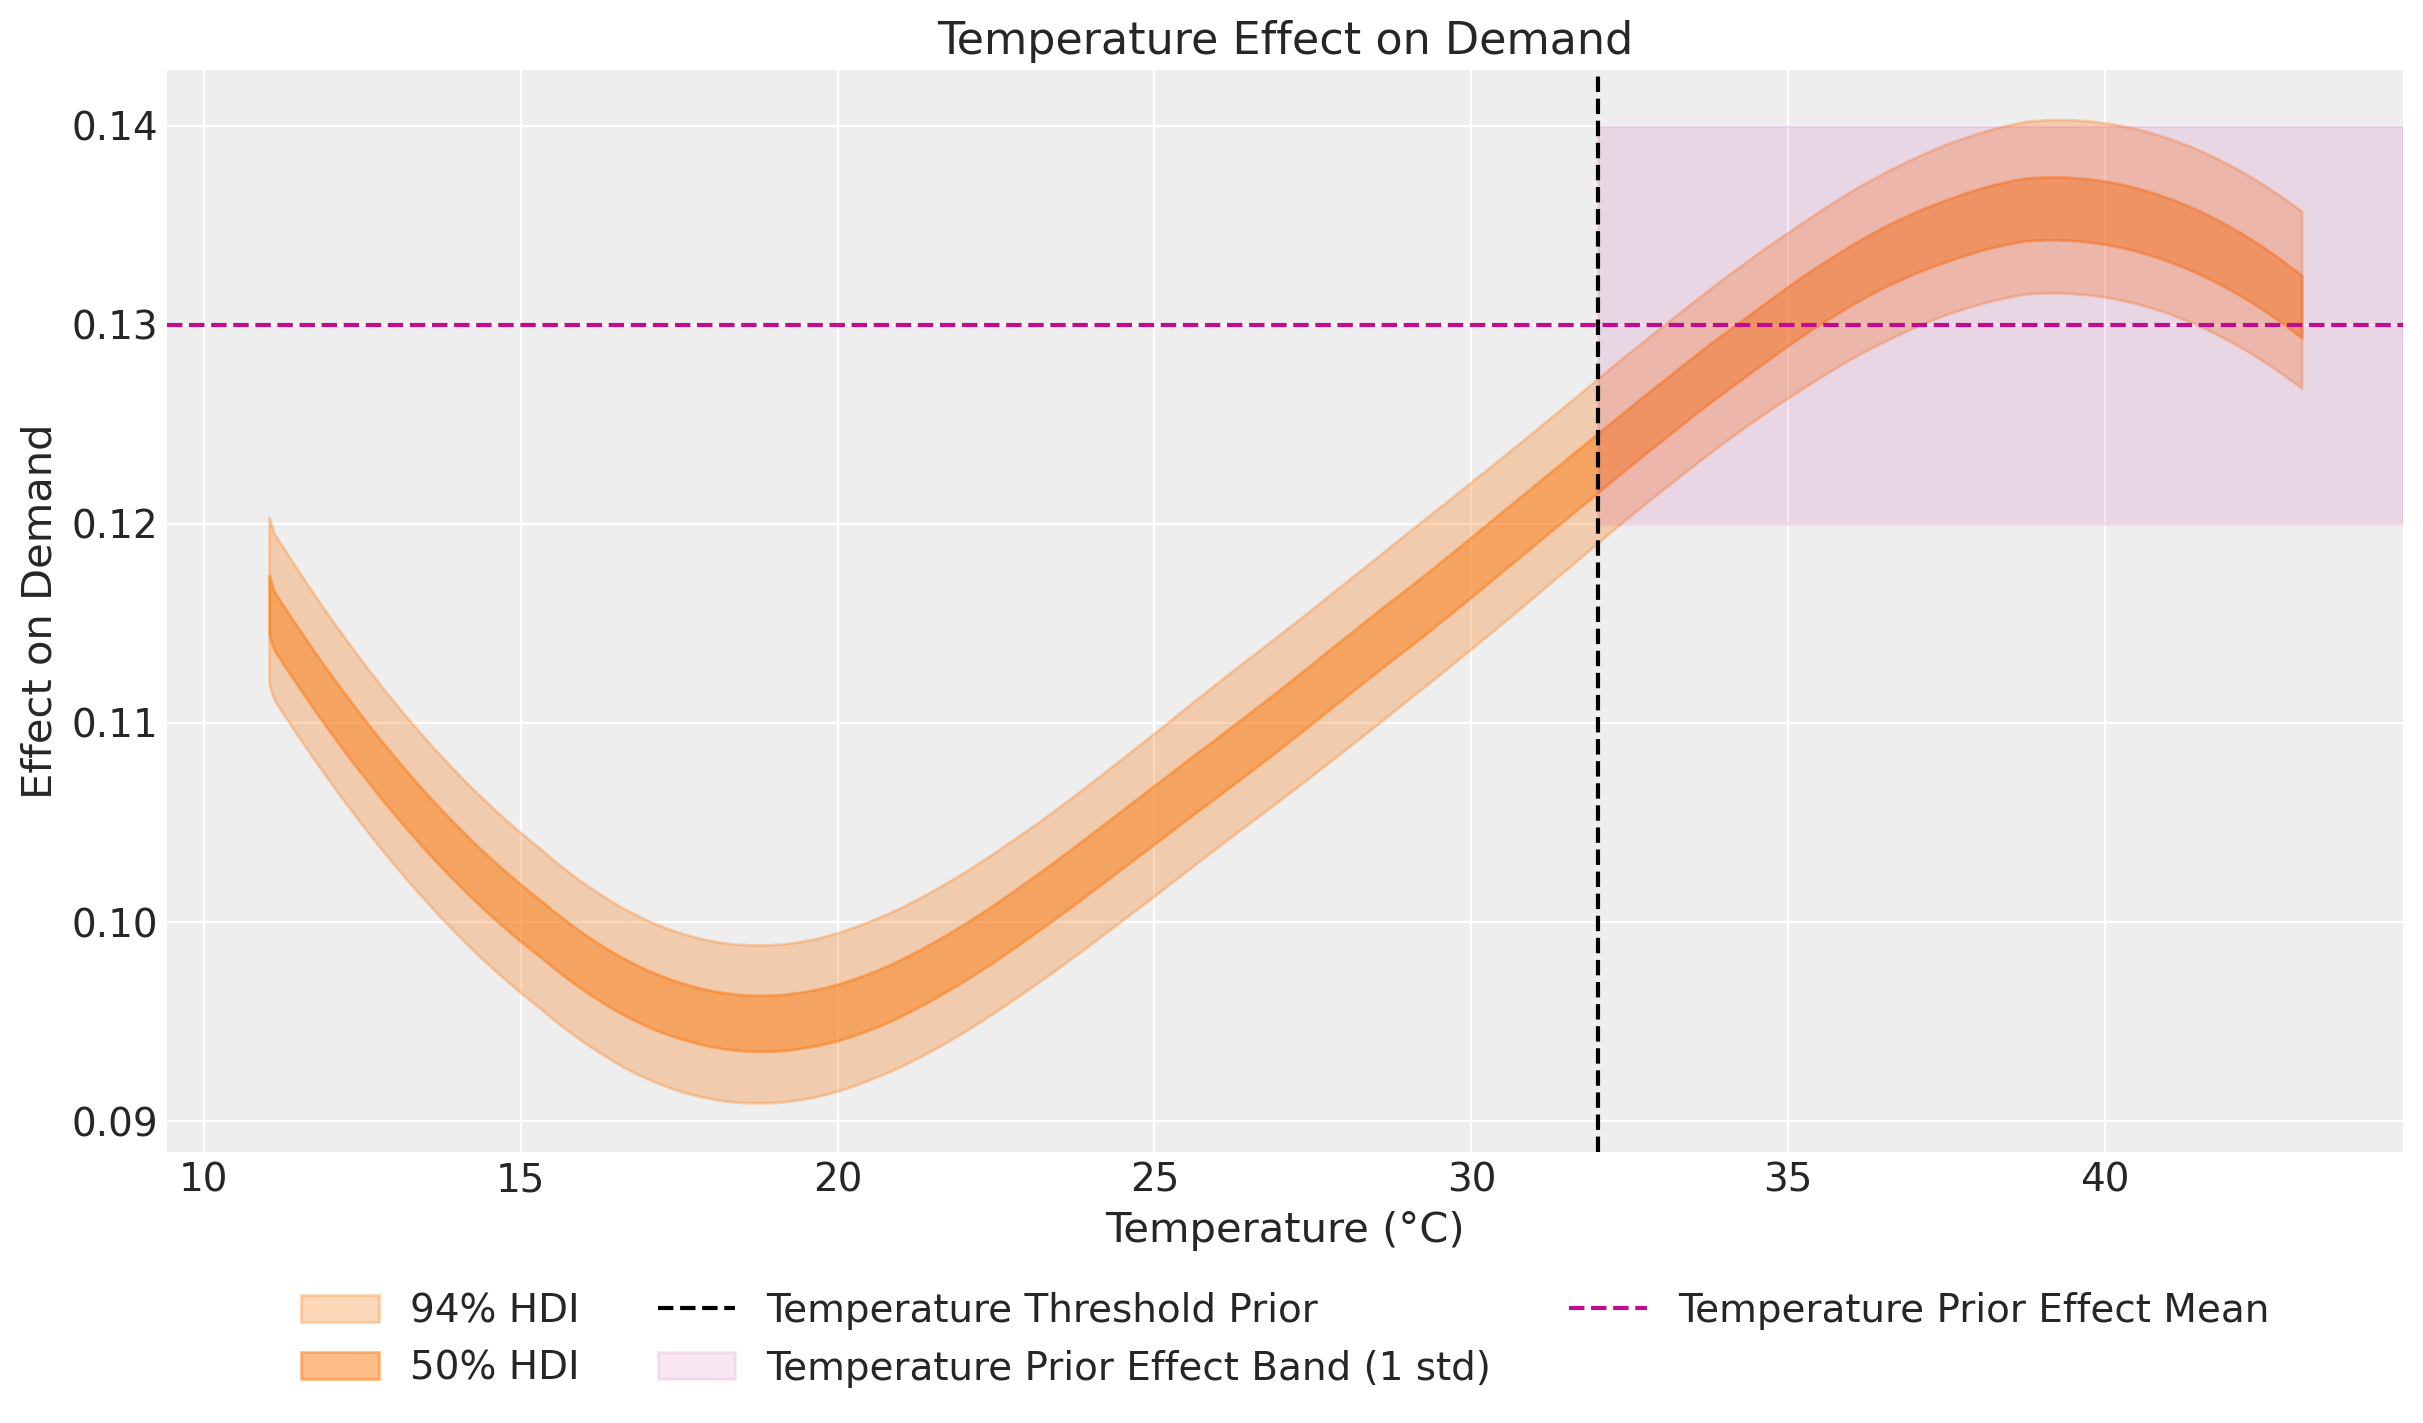
\includegraphics[width=0.95\linewidth]{electricity_forecast_with_priors_32_0.png}
\caption{Calibration of the electricity demand model via an additional likelihood that anchors the temperature-response curve at an expert-elicited reference point. The calibrated posterior (right) is meaningfully tighter than the uncalibrated one (left) while remaining consistent with the historical data.}
\label{fig:calib}
\end{figure}

Two features of this pattern are worth emphasizing in an open-source forecasting context. First, it does not require new framework features. It uses ordinary \texttt{sample} statements with \texttt{obs=} arguments. Second, the community pedigree of this idea is itself an example of the community layer we discuss in the next section. The pattern crystallized in a Pyro tutorial, was adapted to a NumPyro blog post, was extended to lift-test calibration in marketing-mix modeling \citep{pymc_marketing_lift}, and now flows back into operational forecasting workflows. This is open-source forecasting working as designed.


% =============================================================================
\section{The Community Layer}
\label{sec:community}
% =============================================================================

The discussion so far has alternated between framework primitives and worked examples. That alternation is not incidental. Open-source forecasting is increasingly a two-layer story. The lower layer is composed of libraries: the substrates such as NumPyro, the pre-packaged forecasters such as the Nixtla ecosystem and sktime, the deep-learning forecasters such as GluonTS, and the classical statistical toolkits such as statsmodels \citep{nixtla2024, loning2019sktime, alexandrov2020gluonts, statsmodels}. The upper layer is composed of community content: tutorials, blog posts, accompanying notebooks, conference talks, forum threads, starter kits, and book-length open-access texts \citep{hyndman2021forecasting, svetunkov2023adam}.

For a substrate-style library, the upper layer is not optional. The framework primitives alone do not tell a practitioner how to fit a hierarchical state-space model to thousands of intermittent series, how to encode availability constraints in a TSB-style transition, or how to combine a state-space backbone with an HSGP covariate effect. Each of those is a recipe, and recipes live in the upper layer. The case studies surveyed in Section~\ref{sec:cases} are themselves entries in that upper layer. Together with the Pyro forecasting tutorials \citep{pyro_dlm_tutorial}, the Pyro-M5 Starter Kit \citep{pyro_m5_starter}, third-party expositions of censored demand \citep{caron_censored} and intermittent zeros \citep{svetunkov_zeros}, and integrations with adjacent open-source projects \citep{pymc_marketing_lift, orduz_pymc_labs}, they form an ecosystem of recipes that turns substrate primitives into reproducible forecasting workflows.

The NumPyro and Pyro documentation sites themselves carry an extensive collection of tutorials, and the personal blog repository underpinning many of the case studies above \citep{orduz_pymc_labs} is, in practice, a living catalog of patterns. Treating this layer as a peer of the framework layer changes how we should evaluate open-source forecasting tools. A library with strong primitives but no recipes is hard to adopt. A library with excellent recipes but rigid primitives is hard to extend. The healthiest ecosystems invest in both, and a paper that surveys them must acknowledge the recipe layer explicitly.

A practical implication for new contributors is that adding a clear worked example is often the highest-leverage contribution one can make to a probabilistic-programming forecasting ecosystem. New users do not start from the API reference; they start from the tutorial that solves a problem similar to theirs.


% =============================================================================
\section{Discussion and Limitations}
\label{sec:discussion}
% =============================================================================

\paragraph{The learning curve.}
Building probabilistic forecasting models in NumPyro has a steep learning curve. A practitioner needs to be comfortable with JAX semantics, with Bayesian modeling fundamentals, and with the particular \texttt{scan} and \texttt{plate} programming style that recurs across forecasting use cases. This barrier is real, and we do not want to understate it. There is, however, a compensating payoff on the other side of the curve. Because a NumPyro model is just JAX, almost any building block from the \texttt{jax}, \texttt{numpy}, or \texttt{scipy} world can be wired into a model, so a practitioner who hits an unusual requirement is rarely left waiting for a feature to arrive upstream. The effort spent climbing the curve buys an unusually large space of models that can be expressed. The mitigation is the community layer described in Section~\ref{sec:community}. The growing body of worked examples, tutorials, and accompanying notebooks lowers the barrier by giving newcomers concrete starting points to imitate and adapt rather than blank pages to fill. This paper itself is intended as part of that effort, and we would encourage anyone working on probabilistic forecasting models to publish their own worked examples, however small. Every additional recipe shortens the path for the next reader.

\paragraph{When a turn-key library is the right answer.}
A composable substrate is the right tool when the modeling assumption is the central design decision. For many forecasting problems, the modeling assumption is already settled and the operational concerns dominate: a friendly API, robust default hyperparameters, integrated cross-validation, model selection, and deployment tooling matter more than the ability to write a one-off custom likelihood. There is also a production reality: engineering teams often want a stable \texttt{fit} and \texttt{predict} surface they can deploy and monitor, and wrapping a bespoke NumPyro model in that kind of interface is extra work that a packaged library provides out of the box. For a forecasting-research audience this may weigh less than it does in industry, but it is a genuine cost of the substrate approach. In those cases the right tools are pre-packaged forecasting libraries with user-friendly interfaces: the Nixtla ecosystem (\texttt{statsforecast}, \texttt{neuralforecast}, \texttt{hierarchicalforecast}, \texttt{mlforecast}), sktime, GluonTS, and statsmodels \citep{nixtla2024, loning2019sktime, alexandrov2020gluonts, statsmodels}. This is a short illustrative list and many other pre-packaged open-source alternatives exist across the R, Python, and Julia ecosystems. The point is not that one of these layers is superior. The point is that they occupy different positions in a complementary stack, and a healthy forecasting practice draws on whichever layer matches the problem at hand.

\paragraph{Open problems.}
Three open problems strike us as particularly relevant for the substrate-plus-community model of open-source forecasting. First, evaluation and benchmarking. There is no widely adopted benchmark suite that targets the kind of model the substrate makes natural, namely custom likelihoods, hierarchical structures, and prior calibration. The major forecasting competitions reward best-effort accuracy on standard data sets and do not directly reward the modeling flexibility that distinguishes a substrate from a library. Second, integration with large pretrained forecasters. As large time-series foundation models become available, the question of how a probabilistic substrate composes with them, for example by using a pretrained model as an informative prior, is largely open. As noted in Section~\ref{sec:ecosystem}, JAX-native checkpoints and ports such as \texttt{chronos2-jax} \citep{chronos2jax} already make a frozen forecaster callable from JAX, but wrapping one in calibrated Bayesian uncertainty remains unresolved. Third, end-to-end probabilistic decision tooling. A posterior is only as useful as the downstream decision it supports, and the open-source landscape for translating posterior predictives into decisions under loss is far less mature than the landscape for producing the posteriors themselves.

\paragraph{Threats to validity.}
The case studies surveyed in Section~\ref{sec:cases} are illustrative rather than exhaustive. They reflect models we have built and published in the course of practitioner-facing writing, and they are biased toward the patterns we have found useful. A different practitioner working in a different domain would surface different patterns. Our argument is therefore about plausibility and breadth: the same small set of primitives recurs across a wide variety of forecasting problems, which is evidence that the substrate is well factored, not a claim that any particular case study is the optimal solution to its underlying problem.


% =============================================================================
\section{Conclusion}
\label{sec:conclusion}
% =============================================================================

Open-source forecasting benefits from a layered view. Pre-packaged libraries solve standard problems behind friendly APIs. Composable probabilistic substrates such as NumPyro solve nonstandard problems through programmable primitives. The community layer of tutorials and worked examples connects the two. We have argued that this layered view is the right way to position the JAX ecosystem for forecasting. Our emphasis throughout has been the intersection of software and forecasting: how the distinctive demands of forecasting problems, including recursive state, grouped panels, censoring, and structured covariates, shape the design philosophy, the software architecture, and the user-facing interfaces of a composable substrate, rather than a catalog of any one library's features. We have walked through the small set of NumPyro primitives that matter for time series, the inference toolkit that ties them to the broader JAX ecosystem through Optax, and six case studies that exercise the resulting flexibility across hierarchical, intermittent, censored, multivariate, smooth, and calibration settings. The steep learning curve is real, and is being addressed by an active community of recipe writers. None of the ideas in this paper would have been possible without the upstream design choices made by the Pyro project and the JAX ecosystem; the worked examples surveyed here are our contribution to the upper layer of the same stack.


% =============================================================================
\section*{Acknowledgements}
% =============================================================================

This work stands on the shoulders of the open-source probabilistic-programming community. The authors thank the Pyro maintainers, including Eli Bingham, Fritz Obermeyer, Neeraj Pradhan, Martin Jankowiak, and many others, for the design choices and forecasting infrastructure on which NumPyro is built. The authors thank the NumPyro core team, in particular Neeraj Pradhan and Martin Jankowiak, for their ongoing maintenance and stewardship of the project. The JAX team and the broader DeepMind JAX ecosystem, including the Optax and Flax maintainers, provide the numerical foundations that make this work practical at scale. Finally, the authors thank the wider open-source forecasting and probabilistic-programming community, including the readers, commenters, issue reporters, and fellow practitioners whose feedback over many blog posts shaped the case studies surveyed in this paper. Any remaining errors are the authors' alone.


% Bibliography.
\bibliography{refs}

\end{document}
